\documentclass[twoside]{article}

% Packages required by doxygen
\usepackage{fixltx2e}
\usepackage{calc}
\usepackage{doxygen}
\usepackage[export]{adjustbox} % also loads graphicx
\usepackage{graphicx}
\usepackage[utf8]{inputenc}
\usepackage{makeidx}
\usepackage{multicol}
\usepackage{multirow}
\PassOptionsToPackage{warn}{textcomp}
\usepackage{textcomp}
\usepackage[nointegrals]{wasysym}
\usepackage[table]{xcolor}

% Font selection
\usepackage[T1]{fontenc}
\usepackage[scaled=.90]{helvet}
\usepackage{courier}
\usepackage{amssymb}
\usepackage{sectsty}
\renewcommand{\familydefault}{\sfdefault}
\allsectionsfont{%
  \fontseries{bc}\selectfont%
  \color{darkgray}%
}
\renewcommand{\DoxyLabelFont}{%
  \fontseries{bc}\selectfont%
  \color{darkgray}%
}
\newcommand{\+}{\discretionary{\mbox{\scriptsize$\hookleftarrow$}}{}{}}

% Page & text layout
\usepackage{geometry}
\geometry{%
  a4paper,%
  top=2.5cm,%
  bottom=2.5cm,%
  left=2.5cm,%
  right=2.5cm%
}
\tolerance=750
\hfuzz=15pt
\hbadness=750
\setlength{\emergencystretch}{15pt}
\setlength{\parindent}{0cm}
\setlength{\parskip}{3ex plus 2ex minus 2ex}
\makeatletter
\renewcommand{\paragraph}{%
  \@startsection{paragraph}{4}{0ex}{-1.0ex}{1.0ex}{%
    \normalfont\normalsize\bfseries\SS@parafont%
  }%
}
\renewcommand{\subparagraph}{%
  \@startsection{subparagraph}{5}{0ex}{-1.0ex}{1.0ex}{%
    \normalfont\normalsize\bfseries\SS@subparafont%
  }%
}
\makeatother

% Headers & footers
\usepackage{fancyhdr}
\pagestyle{fancyplain}
\fancyhead[LE]{\fancyplain{}{\bfseries\thepage}}
\fancyhead[CE]{\fancyplain{}{}}
\fancyhead[RE]{\fancyplain{}{\bfseries\leftmark}}
\fancyhead[LO]{\fancyplain{}{\bfseries\rightmark}}
\fancyhead[CO]{\fancyplain{}{}}
\fancyhead[RO]{\fancyplain{}{\bfseries\thepage}}
\fancyfoot[LE]{\fancyplain{}{}}
\fancyfoot[CE]{\fancyplain{}{}}
\fancyfoot[RE]{\fancyplain{}{\bfseries\scriptsize Generated by Doxygen }}
\fancyfoot[LO]{\fancyplain{}{\bfseries\scriptsize Generated by Doxygen }}
\fancyfoot[CO]{\fancyplain{}{}}
\fancyfoot[RO]{\fancyplain{}{}}
\renewcommand{\footrulewidth}{0.4pt}
\renewcommand{\sectionmark}[1]{%
  \markright{\thesection\ #1}%
}

% Indices & bibliography
\usepackage{natbib}
\usepackage[titles]{tocloft}
\setcounter{tocdepth}{3}
\setcounter{secnumdepth}{5}
\makeindex

% Hyperlinks (required, but should be loaded last)
\usepackage{ifpdf}
\ifpdf
  \usepackage[pdftex,pagebackref=true]{hyperref}
\else
  \usepackage[ps2pdf,pagebackref=true]{hyperref}
\fi
\hypersetup{%
  colorlinks=true,%
  linkcolor=blue,%
  citecolor=blue,%
  unicode%
}

% Custom commands
\newcommand{\clearemptydoublepage}{%
  \newpage{\pagestyle{empty}\cleardoublepage}%
}

\usepackage{caption}
\captionsetup{labelsep=space,justification=centering,font={bf},singlelinecheck=off,skip=4pt,position=top}

%===== C O N T E N T S =====

\begin{document}

% Titlepage & ToC
\hypersetup{pageanchor=false,
             bookmarksnumbered=true,
             pdfencoding=unicode
            }
\pagenumbering{roman}
\begin{titlepage}
\vspace*{7cm}
\begin{center}%
{\Large P\+A05 }\\
\vspace*{1cm}
{\large Generated by Doxygen 1.8.11}\\
\end{center}
\end{titlepage}
\tableofcontents
\pagenumbering{arabic}
\hypersetup{pageanchor=true}

%--- Begin generated contents ---
\section{Hierarchical Index}
\subsection{Class Hierarchy}
This inheritance list is sorted roughly, but not completely, alphabetically\-:\begin{DoxyCompactList}
\item \contentsline{section}{List\-Interface$<$ Item\-Type $>$}{\pageref{class_list_interface}}{}
\begin{DoxyCompactList}
\item \contentsline{section}{Linked\-List$<$ Item\-Type $>$}{\pageref{class_linked_list}}{}
\end{DoxyCompactList}
\item logic\-\_\-error\begin{DoxyCompactList}
\item \contentsline{section}{Precond\-Violated\-Except}{\pageref{class_precond_violated_except}}{}
\end{DoxyCompactList}
\item \contentsline{section}{Node$<$ Item\-Type $>$}{\pageref{class_node}}{}
\end{DoxyCompactList}

\section{Class Index}
\subsection{Class List}
Here are the classes, structs, unions and interfaces with brief descriptions\-:\begin{DoxyCompactList}
\item\contentsline{section}{\hyperlink{class_linked_list}{Linked\-List$<$ Item\-Type $>$} }{\pageref{class_linked_list}}{}
\item\contentsline{section}{\hyperlink{class_list_interface}{List\-Interface$<$ Item\-Type $>$} }{\pageref{class_list_interface}}{}
\item\contentsline{section}{\hyperlink{class_node}{Node$<$ Item\-Type $>$} }{\pageref{class_node}}{}
\item\contentsline{section}{\hyperlink{class_precond_violated_except}{Precond\-Violated\-Except} }{\pageref{class_precond_violated_except}}{}
\end{DoxyCompactList}

\section{File Index}
\subsection{File List}
Here is a list of all documented files with brief descriptions\+:\begin{DoxyCompactList}
\item\contentsline{section}{\hyperlink{_array_queue_8cpp}{Array\+Queue.\+cpp} }{\pageref{_array_queue_8cpp}}{}
\item\contentsline{section}{\hyperlink{_array_queue_8h}{Array\+Queue.\+h} }{\pageref{_array_queue_8h}}{}
\item\contentsline{section}{{\bfseries Event.\+h} }{\pageref{_event_8h}}{}
\item\contentsline{section}{\hyperlink{_linked_list_8cpp}{Linked\+List.\+cpp} }{\pageref{_linked_list_8cpp}}{}
\item\contentsline{section}{\hyperlink{_linked_list_8h}{Linked\+List.\+h} \\*Header file for a linked list }{\pageref{_linked_list_8h}}{}
\item\contentsline{section}{\hyperlink{_linked_queue_8h}{Linked\+Queue.\+h} }{\pageref{_linked_queue_8h}}{}
\item\contentsline{section}{\hyperlink{_list_interface_8h}{List\+Interface.\+h} \\*Interface file for the List A\+DT }{\pageref{_list_interface_8h}}{}
\item\contentsline{section}{\hyperlink{_node_8cpp}{Node.\+cpp} }{\pageref{_node_8cpp}}{}
\item\contentsline{section}{\hyperlink{_node_8h}{Node.\+h} }{\pageref{_node_8h}}{}
\item\contentsline{section}{\hyperlink{_precond_violated_except_8cpp}{Precond\+Violated\+Except.\+cpp} }{\pageref{_precond_violated_except_8cpp}}{}
\item\contentsline{section}{\hyperlink{_precond_violated_except_8h}{Precond\+Violated\+Except.\+h} }{\pageref{_precond_violated_except_8h}}{}
\item\contentsline{section}{\hyperlink{_priority_queue_interface_8h}{Priority\+Queue\+Interface.\+h} }{\pageref{_priority_queue_interface_8h}}{}
\item\contentsline{section}{\hyperlink{_queue_interface_8h}{Queue\+Interface.\+h} }{\pageref{_queue_interface_8h}}{}
\item\contentsline{section}{\hyperlink{_s_l___priority_queue_8h}{S\+L\+\_\+\+Priority\+Queue.\+h} }{\pageref{_s_l___priority_queue_8h}}{}
\item\contentsline{section}{\hyperlink{_sorted_list_interface_8h}{Sorted\+List\+Interface.\+h} }{\pageref{_sorted_list_interface_8h}}{}
\item\contentsline{section}{\hyperlink{_sorted_list_is_a_8h}{Sorted\+List\+Is\+A.\+h} }{\pageref{_sorted_list_is_a_8h}}{}
\end{DoxyCompactList}

\section{Class Documentation}
\hypertarget{class_array_queue}{}\subsection{Array\+Queue$<$ Item\+Type $>$ Class Template Reference}
\label{class_array_queue}\index{Array\+Queue$<$ Item\+Type $>$@{Array\+Queue$<$ Item\+Type $>$}}
Inheritance diagram for Array\+Queue$<$ Item\+Type $>$\+:\begin{figure}[H]
\begin{center}
\leavevmode
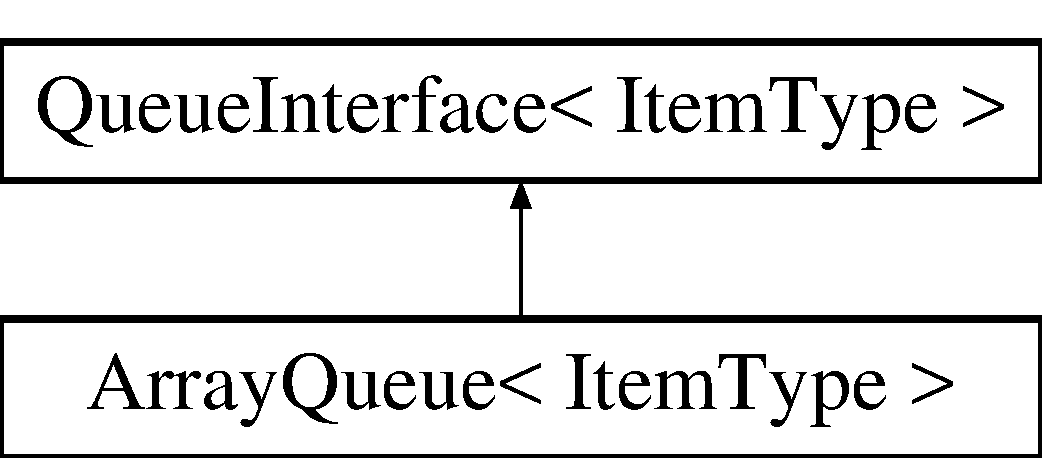
\includegraphics[height=2.000000cm]{class_array_queue}
\end{center}
\end{figure}
\subsubsection*{Public Member Functions}
\begin{DoxyCompactItemize}
\item 
bool \hyperlink{class_array_queue_a9ecf3552d6b73c51f6b81277c6ba453d}{is\+Empty} () const 
\item 
bool \hyperlink{class_array_queue_ae8942e3f72dbbfba821e8d7dabf9ec33}{enqueue} (const Item\+Type \&new\+Entry)
\item 
bool \hyperlink{class_array_queue_a13a06eec37f359d07a785f831e1f287c}{dequeue} ()
\item 
Item\+Type \hyperlink{class_array_queue_aba429775b7eedf84920bb00e78022d8a}{peek\+Front} () const   throw (\+Precond\+Violated\+Except)
\end{DoxyCompactItemize}


\subsubsection{Member Function Documentation}
\index{Array\+Queue@{Array\+Queue}!dequeue@{dequeue}}
\index{dequeue@{dequeue}!Array\+Queue@{Array\+Queue}}
\paragraph[{\texorpdfstring{dequeue()}{dequeue()}}]{\setlength{\rightskip}{0pt plus 5cm}template$<$class Item\+Type $>$ bool {\bf Array\+Queue}$<$ Item\+Type $>$\+::dequeue (
\begin{DoxyParamCaption}
{}
\end{DoxyParamCaption}
)\hspace{0.3cm}{\ttfamily [virtual]}}\hypertarget{class_array_queue_a13a06eec37f359d07a785f831e1f287c}{}\label{class_array_queue_a13a06eec37f359d07a785f831e1f287c}
Removes the front of this queue. \begin{DoxyPostcond}{Postcondition}
If the operation was successful, the front of the queue has been removed. 
\end{DoxyPostcond}
\begin{DoxyReturn}{Returns}
True if the removal is successful or false if not. 
\end{DoxyReturn}


Implements \hyperlink{class_queue_interface_a0d0d1b1a8b84bee0c3d8c4798a95e792}{Queue\+Interface$<$ Item\+Type $>$}.

\index{Array\+Queue@{Array\+Queue}!enqueue@{enqueue}}
\index{enqueue@{enqueue}!Array\+Queue@{Array\+Queue}}
\paragraph[{\texorpdfstring{enqueue(const Item\+Type \&new\+Entry)}{enqueue(const ItemType &newEntry)}}]{\setlength{\rightskip}{0pt plus 5cm}template$<$class Item\+Type $>$ bool {\bf Array\+Queue}$<$ Item\+Type $>$\+::enqueue (
\begin{DoxyParamCaption}
\item[{const Item\+Type \&}]{new\+Entry}
\end{DoxyParamCaption}
)\hspace{0.3cm}{\ttfamily [virtual]}}\hypertarget{class_array_queue_ae8942e3f72dbbfba821e8d7dabf9ec33}{}\label{class_array_queue_ae8942e3f72dbbfba821e8d7dabf9ec33}
Adds a new entry to the back of this queue. \begin{DoxyPostcond}{Postcondition}
If the operation was successful, new\+Entry is at the back of the queue. 
\end{DoxyPostcond}

\begin{DoxyParams}{Parameters}
{\em new\+Entry} & The object to be added as a new entry. \\
\hline
\end{DoxyParams}
\begin{DoxyReturn}{Returns}
True if the addition is successful or false if not. 
\end{DoxyReturn}


Implements \hyperlink{class_queue_interface_af65d0ec8ce74a1c03ba83ba569cb7c14}{Queue\+Interface$<$ Item\+Type $>$}.

\index{Array\+Queue@{Array\+Queue}!is\+Empty@{is\+Empty}}
\index{is\+Empty@{is\+Empty}!Array\+Queue@{Array\+Queue}}
\paragraph[{\texorpdfstring{is\+Empty() const }{isEmpty() const }}]{\setlength{\rightskip}{0pt plus 5cm}template$<$class Item\+Type $>$ bool {\bf Array\+Queue}$<$ Item\+Type $>$\+::is\+Empty (
\begin{DoxyParamCaption}
{}
\end{DoxyParamCaption}
) const\hspace{0.3cm}{\ttfamily [virtual]}}\hypertarget{class_array_queue_a9ecf3552d6b73c51f6b81277c6ba453d}{}\label{class_array_queue_a9ecf3552d6b73c51f6b81277c6ba453d}
Sees whether this queue is empty. \begin{DoxyReturn}{Returns}
True if the queue is empty, or false if not. 
\end{DoxyReturn}


Implements \hyperlink{class_queue_interface_adfc78ad2af130ad5f0867de0e9f63ec7}{Queue\+Interface$<$ Item\+Type $>$}.

\index{Array\+Queue@{Array\+Queue}!peek\+Front@{peek\+Front}}
\index{peek\+Front@{peek\+Front}!Array\+Queue@{Array\+Queue}}
\paragraph[{\texorpdfstring{peek\+Front() const }{peekFront() const }}]{\setlength{\rightskip}{0pt plus 5cm}template$<$class Item\+Type $>$ Item\+Type {\bf Array\+Queue}$<$ Item\+Type $>$\+::peek\+Front (
\begin{DoxyParamCaption}
{}
\end{DoxyParamCaption}
) const throw  {\bf Precond\+Violated\+Except}) \hspace{0.3cm}{\ttfamily [virtual]}}\hypertarget{class_array_queue_aba429775b7eedf84920bb00e78022d8a}{}\label{class_array_queue_aba429775b7eedf84920bb00e78022d8a}

\begin{DoxyExceptions}{Exceptions}
{\em \hyperlink{class_precond_violated_except}{Precond\+Violated\+Except}} & if queue is empty. \\
\hline
\end{DoxyExceptions}


Implements \hyperlink{class_queue_interface_a9a6097cc3742158736ef0908586e2066}{Queue\+Interface$<$ Item\+Type $>$}.



The documentation for this class was generated from the following files\+:\begin{DoxyCompactItemize}
\item 
\hyperlink{_array_queue_8h}{Array\+Queue.\+h}\item 
\hyperlink{_array_queue_8cpp}{Array\+Queue.\+cpp}\end{DoxyCompactItemize}

\hypertarget{class_event}{}\subsection{Event Class Reference}
\label{class_event}\index{Event@{Event}}
\subsubsection*{Public Member Functions}
\begin{DoxyCompactItemize}
\item 
bool {\bfseries operator==} (const \hyperlink{class_event}{Event} \&right\+Side) const \hypertarget{class_event_aeeee52bac39d185809bfc342a25be2c0}{}\label{class_event_aeeee52bac39d185809bfc342a25be2c0}

\item 
bool {\bfseries operator!=} (const \hyperlink{class_event}{Event} \&right\+Side) const \hypertarget{class_event_adfc8aa073d2ca536ac2ba3d8a5c15038}{}\label{class_event_adfc8aa073d2ca536ac2ba3d8a5c15038}

\item 
bool {\bfseries operator$>$} (const \hyperlink{class_event}{Event} \&right\+Side) const \hypertarget{class_event_af1b0cac6dc643b7fdeaa13f6fb4ccf31}{}\label{class_event_af1b0cac6dc643b7fdeaa13f6fb4ccf31}

\item 
bool {\bfseries operator$<$} (const \hyperlink{class_event}{Event} \&right\+Side) const \hypertarget{class_event_ab79729abd53ca25f0424d48600ce9ee6}{}\label{class_event_ab79729abd53ca25f0424d48600ce9ee6}

\item 
bool {\bfseries operator=} (const \hyperlink{class_event}{Event} \&right\+Side)\hypertarget{class_event_a56ba06376a5dd7890c80a23b33fc2474}{}\label{class_event_a56ba06376a5dd7890c80a23b33fc2474}

\end{DoxyCompactItemize}
\subsubsection*{Public Attributes}
\begin{DoxyCompactItemize}
\item 
bool {\bfseries arrival}\hypertarget{class_event_ae018eaef21b64be859ac1f87d5cf8e40}{}\label{class_event_ae018eaef21b64be859ac1f87d5cf8e40}

\item 
int {\bfseries time}\hypertarget{class_event_ad4c0fbb00c3fd993405df98bafcd52c5}{}\label{class_event_ad4c0fbb00c3fd993405df98bafcd52c5}

\item 
int {\bfseries length}\hypertarget{class_event_a1d58d4227e70762d73683ab5eac7e17a}{}\label{class_event_a1d58d4227e70762d73683ab5eac7e17a}

\end{DoxyCompactItemize}


The documentation for this class was generated from the following files\+:\begin{DoxyCompactItemize}
\item 
Event.\+h\item 
Event.\+cpp\end{DoxyCompactItemize}

\hypertarget{class_linked_list}{}\subsection{Linked\+List$<$ Item\+Type $>$ Class Template Reference}
\label{class_linked_list}\index{Linked\+List$<$ Item\+Type $>$@{Linked\+List$<$ Item\+Type $>$}}
Inheritance diagram for Linked\+List$<$ Item\+Type $>$\+:\begin{figure}[H]
\begin{center}
\leavevmode
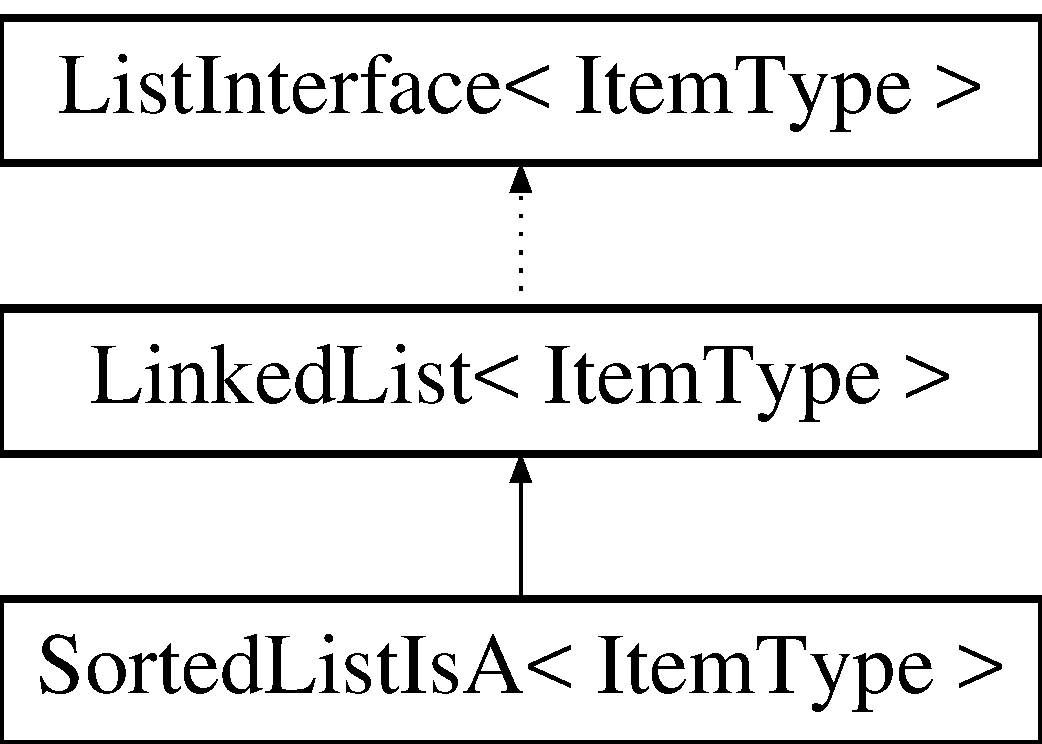
\includegraphics[height=3.000000cm]{class_linked_list}
\end{center}
\end{figure}
\subsubsection*{Public Member Functions}
\begin{DoxyCompactItemize}
\item 
\hyperlink{class_linked_list_adf8d8164e06b6d358a36df7e53e814ee}{Linked\+List} ()
\item 
\hyperlink{class_linked_list_a6f1443c6120352f1f5b6bd3c0d95e41e}{Linked\+List} (const \hyperlink{class_linked_list}{Linked\+List}$<$ Item\+Type $>$ \&a\+List)
\item 
virtual \hyperlink{class_linked_list_a66aee17d756fe0e002375897383c180b}{$\sim$\+Linked\+List} ()
\item 
bool \hyperlink{class_linked_list_adb17aed0ceacbbe1f247d235f491f0d5}{is\+Empty} () const 
\item 
int \hyperlink{class_linked_list_adae55d6b79235c816cb9e05027fd2e7a}{get\+Length} () const 
\item 
bool \hyperlink{class_linked_list_ae8a19375505e87e2e4fc0e9b5afe4d4d}{insert} (int new\+Position, const Item\+Type \&new\+Entry)
\item 
bool \hyperlink{class_linked_list_a16a02716b5b2efb6fb1e3d18721b53e4}{remove} (int position)
\item 
void \hyperlink{class_linked_list_a7d1d9cf83eef67b6c4d700a3cc5970e1}{clear} ()
\item 
Item\+Type \hyperlink{class_linked_list_a79f005e696c19f6ccf90d9d535afa999}{get\+Entry} (int position) const   throw (\+Precond\+Violated\+Except)
\item 
void \hyperlink{class_linked_list_a3035f880c50e7d8f68e67c093d4607ca}{replace} (int position, const Item\+Type \&new\+Entry)  throw (\+Precond\+Violated\+Except)
\end{DoxyCompactItemize}


\subsubsection{Constructor \& Destructor Documentation}
\index{Linked\+List@{Linked\+List}!Linked\+List@{Linked\+List}}
\index{Linked\+List@{Linked\+List}!Linked\+List@{Linked\+List}}
\paragraph[{\texorpdfstring{Linked\+List()}{LinkedList()}}]{\setlength{\rightskip}{0pt plus 5cm}template$<$class Item\+Type $>$ {\bf Linked\+List}$<$ Item\+Type $>$\+::{\bf Linked\+List} (
\begin{DoxyParamCaption}
{}
\end{DoxyParamCaption}
)}\hypertarget{class_linked_list_adf8d8164e06b6d358a36df7e53e814ee}{}\label{class_linked_list_adf8d8164e06b6d358a36df7e53e814ee}
default constructor \index{Linked\+List@{Linked\+List}!Linked\+List@{Linked\+List}}
\index{Linked\+List@{Linked\+List}!Linked\+List@{Linked\+List}}
\paragraph[{\texorpdfstring{Linked\+List(const Linked\+List$<$ Item\+Type $>$ \&a\+List)}{LinkedList(const LinkedList< ItemType > &aList)}}]{\setlength{\rightskip}{0pt plus 5cm}template$<$class Item\+Type $>$ {\bf Linked\+List}$<$ Item\+Type $>$\+::{\bf Linked\+List} (
\begin{DoxyParamCaption}
\item[{const {\bf Linked\+List}$<$ Item\+Type $>$ \&}]{a\+List}
\end{DoxyParamCaption}
)}\hypertarget{class_linked_list_a6f1443c6120352f1f5b6bd3c0d95e41e}{}\label{class_linked_list_a6f1443c6120352f1f5b6bd3c0d95e41e}
copy constructor \index{Linked\+List@{Linked\+List}!````~Linked\+List@{$\sim$\+Linked\+List}}
\index{````~Linked\+List@{$\sim$\+Linked\+List}!Linked\+List@{Linked\+List}}
\paragraph[{\texorpdfstring{$\sim$\+Linked\+List()}{~LinkedList()}}]{\setlength{\rightskip}{0pt plus 5cm}template$<$class Item\+Type $>$ {\bf Linked\+List}$<$ Item\+Type $>$\+::$\sim${\bf Linked\+List} (
\begin{DoxyParamCaption}
{}
\end{DoxyParamCaption}
)\hspace{0.3cm}{\ttfamily [virtual]}}\hypertarget{class_linked_list_a66aee17d756fe0e002375897383c180b}{}\label{class_linked_list_a66aee17d756fe0e002375897383c180b}
destructor 

\subsubsection{Member Function Documentation}
\index{Linked\+List@{Linked\+List}!clear@{clear}}
\index{clear@{clear}!Linked\+List@{Linked\+List}}
\paragraph[{\texorpdfstring{clear()}{clear()}}]{\setlength{\rightskip}{0pt plus 5cm}template$<$class Item\+Type $>$ void {\bf Linked\+List}$<$ Item\+Type $>$\+::clear (
\begin{DoxyParamCaption}
{}
\end{DoxyParamCaption}
)\hspace{0.3cm}{\ttfamily [virtual]}}\hypertarget{class_linked_list_a7d1d9cf83eef67b6c4d700a3cc5970e1}{}\label{class_linked_list_a7d1d9cf83eef67b6c4d700a3cc5970e1}
removes all items from the list. \begin{DoxyPrecond}{Precondition}
None. 
\end{DoxyPrecond}
\begin{DoxyPostcond}{Postcondition}
List contains no entries. 
\end{DoxyPostcond}


Implements \hyperlink{class_list_interface_adfda414908b645bdf19bcab8269168b7}{List\+Interface$<$ Item\+Type $>$}.

\index{Linked\+List@{Linked\+List}!get\+Entry@{get\+Entry}}
\index{get\+Entry@{get\+Entry}!Linked\+List@{Linked\+List}}
\paragraph[{\texorpdfstring{get\+Entry(int position) const }{getEntry(int position) const }}]{\setlength{\rightskip}{0pt plus 5cm}template$<$class Item\+Type $>$ Item\+Type {\bf Linked\+List}$<$ Item\+Type $>$\+::get\+Entry (
\begin{DoxyParamCaption}
\item[{int}]{position}
\end{DoxyParamCaption}
) const throw  {\bf Precond\+Violated\+Except}) \hspace{0.3cm}{\ttfamily [virtual]}}\hypertarget{class_linked_list_a79f005e696c19f6ccf90d9d535afa999}{}\label{class_linked_list_a79f005e696c19f6ccf90d9d535afa999}
Gets the entry at the given position in this list. \begin{DoxyPrecond}{Precondition}
1 $<$= position $<$= \hyperlink{class_linked_list_adae55d6b79235c816cb9e05027fd2e7a}{get\+Length()}. 
\end{DoxyPrecond}
\begin{DoxyPostcond}{Postcondition}
The desired entry has been returned. 
\end{DoxyPostcond}

\begin{DoxyParams}{Parameters}
{\em position} & The list position of the desired entry. \\
\hline
\end{DoxyParams}
\begin{DoxyReturn}{Returns}
The entry at the given position. 
\end{DoxyReturn}

\begin{DoxyExceptions}{Exceptions}
{\em \hyperlink{class_precond_violated_except}{Precond\+Violated\+Except}} & if position $<$ 1 or position $>$ \hyperlink{class_linked_list_adae55d6b79235c816cb9e05027fd2e7a}{get\+Length()}. \\
\hline
\end{DoxyExceptions}


Implements \hyperlink{class_list_interface_a86987f69e5056d287212ede41db1956a}{List\+Interface$<$ Item\+Type $>$}.

\index{Linked\+List@{Linked\+List}!get\+Length@{get\+Length}}
\index{get\+Length@{get\+Length}!Linked\+List@{Linked\+List}}
\paragraph[{\texorpdfstring{get\+Length() const }{getLength() const }}]{\setlength{\rightskip}{0pt plus 5cm}template$<$class Item\+Type $>$ int {\bf Linked\+List}$<$ Item\+Type $>$\+::get\+Length (
\begin{DoxyParamCaption}
{}
\end{DoxyParamCaption}
) const\hspace{0.3cm}{\ttfamily [virtual]}}\hypertarget{class_linked_list_adae55d6b79235c816cb9e05027fd2e7a}{}\label{class_linked_list_adae55d6b79235c816cb9e05027fd2e7a}
checks how many items are in the list \begin{DoxyReturn}{Returns}
the integer value of how many items are contained in the list. 
\end{DoxyReturn}


Implements \hyperlink{class_list_interface_afc85695d4137f1e29ff02e179c9f3221}{List\+Interface$<$ Item\+Type $>$}.

\index{Linked\+List@{Linked\+List}!insert@{insert}}
\index{insert@{insert}!Linked\+List@{Linked\+List}}
\paragraph[{\texorpdfstring{insert(int new\+Position, const Item\+Type \&new\+Entry)}{insert(int newPosition, const ItemType &newEntry)}}]{\setlength{\rightskip}{0pt plus 5cm}template$<$class Item\+Type $>$ bool {\bf Linked\+List}$<$ Item\+Type $>$\+::insert (
\begin{DoxyParamCaption}
\item[{int}]{new\+Position, }
\item[{const Item\+Type \&}]{new\+Entry}
\end{DoxyParamCaption}
)\hspace{0.3cm}{\ttfamily [virtual]}}\hypertarget{class_linked_list_ae8a19375505e87e2e4fc0e9b5afe4d4d}{}\label{class_linked_list_ae8a19375505e87e2e4fc0e9b5afe4d4d}
inserts an entry into the list at a given position \begin{DoxyPrecond}{Precondition}
None. 
\end{DoxyPrecond}
\begin{DoxyPostcond}{Postcondition}
if the position is valid and insertion is possible a new entry is entered into the list. 
\end{DoxyPostcond}

\begin{DoxyParams}{Parameters}
{\em new\+Position} & the position in the list at which to insert the new entry. \\
\hline
{\em new\+Entry} & the new item to be placed in the list. \\
\hline
\end{DoxyParams}
\begin{DoxyReturn}{Returns}
True if the item was successfully placed in the list. 
\end{DoxyReturn}


Implements \hyperlink{class_list_interface_a5b2f86954a86172699a3495982c38e77}{List\+Interface$<$ Item\+Type $>$}.



Reimplemented in \hyperlink{class_sorted_list_is_a_aa80ef5215183e3a17f2a2f2e76d4fca3}{Sorted\+List\+Is\+A$<$ Item\+Type $>$}.

\index{Linked\+List@{Linked\+List}!is\+Empty@{is\+Empty}}
\index{is\+Empty@{is\+Empty}!Linked\+List@{Linked\+List}}
\paragraph[{\texorpdfstring{is\+Empty() const }{isEmpty() const }}]{\setlength{\rightskip}{0pt plus 5cm}template$<$class Item\+Type $>$ bool {\bf Linked\+List}$<$ Item\+Type $>$\+::is\+Empty (
\begin{DoxyParamCaption}
{}
\end{DoxyParamCaption}
) const\hspace{0.3cm}{\ttfamily [virtual]}}\hypertarget{class_linked_list_adb17aed0ceacbbe1f247d235f491f0d5}{}\label{class_linked_list_adb17aed0ceacbbe1f247d235f491f0d5}
checks if the list contains any items \begin{DoxyReturn}{Returns}
returns true if the list is empty. 
\end{DoxyReturn}


Implements \hyperlink{class_list_interface_a924f91e7f81d7dcd3fda79bbcc671394}{List\+Interface$<$ Item\+Type $>$}.

\index{Linked\+List@{Linked\+List}!remove@{remove}}
\index{remove@{remove}!Linked\+List@{Linked\+List}}
\paragraph[{\texorpdfstring{remove(int position)}{remove(int position)}}]{\setlength{\rightskip}{0pt plus 5cm}template$<$class Item\+Type $>$ bool {\bf Linked\+List}$<$ Item\+Type $>$\+::remove (
\begin{DoxyParamCaption}
\item[{int}]{position}
\end{DoxyParamCaption}
)\hspace{0.3cm}{\ttfamily [virtual]}}\hypertarget{class_linked_list_a16a02716b5b2efb6fb1e3d18721b53e4}{}\label{class_linked_list_a16a02716b5b2efb6fb1e3d18721b53e4}
removes the entry at the specified position. \begin{DoxyPrecond}{Precondition}
None. 
\end{DoxyPrecond}
\begin{DoxyPostcond}{Postcondition}
if the position is valid the item is removed from the list and the list is renumbered. 
\end{DoxyPostcond}

\begin{DoxyParams}{Parameters}
{\em position} & the position in the list which contains the item to be removed. \\
\hline
\end{DoxyParams}
\begin{DoxyReturn}{Returns}
True if the item was removed succesfully otherwise returns false. 
\end{DoxyReturn}


Implements \hyperlink{class_list_interface_a5543002ec0d64bd2a63f3732f437af65}{List\+Interface$<$ Item\+Type $>$}.

\index{Linked\+List@{Linked\+List}!replace@{replace}}
\index{replace@{replace}!Linked\+List@{Linked\+List}}
\paragraph[{\texorpdfstring{replace(int position, const Item\+Type \&new\+Entry)}{replace(int position, const ItemType &newEntry)}}]{\setlength{\rightskip}{0pt plus 5cm}template$<$class Item\+Type $>$ void {\bf Linked\+List}$<$ Item\+Type $>$\+::replace (
\begin{DoxyParamCaption}
\item[{int}]{position, }
\item[{const Item\+Type \&}]{new\+Entry}
\end{DoxyParamCaption}
) throw  {\bf Precond\+Violated\+Except}) \hspace{0.3cm}{\ttfamily [virtual]}}\hypertarget{class_linked_list_a3035f880c50e7d8f68e67c093d4607ca}{}\label{class_linked_list_a3035f880c50e7d8f68e67c093d4607ca}
Replaces the entry at the given position in this list. \begin{DoxyPrecond}{Precondition}
1 $<$= position $<$= \hyperlink{class_linked_list_adae55d6b79235c816cb9e05027fd2e7a}{get\+Length()}. 
\end{DoxyPrecond}
\begin{DoxyPostcond}{Postcondition}
The entry at the given position is new\+Entry. 
\end{DoxyPostcond}

\begin{DoxyParams}{Parameters}
{\em position} & The list position of the entry to replace. \\
\hline
{\em new\+Entry} & The replacement entry. \\
\hline
\end{DoxyParams}

\begin{DoxyExceptions}{Exceptions}
{\em \hyperlink{class_precond_violated_except}{Precond\+Violated\+Except}} & if position $<$ 1 or position $>$ \hyperlink{class_linked_list_adae55d6b79235c816cb9e05027fd2e7a}{get\+Length()}. \\
\hline
\end{DoxyExceptions}


Implements \hyperlink{class_list_interface_aae877a56b7b9f5f526c37a00e234fad1}{List\+Interface$<$ Item\+Type $>$}.



Reimplemented in \hyperlink{class_sorted_list_is_a_ae85cca0f8a4a306d6d28cc5993e5895c}{Sorted\+List\+Is\+A$<$ Item\+Type $>$}.



The documentation for this class was generated from the following files\+:\begin{DoxyCompactItemize}
\item 
\hyperlink{_linked_list_8h}{Linked\+List.\+h}\item 
\hyperlink{_linked_list_8cpp}{Linked\+List.\+cpp}\end{DoxyCompactItemize}

\hypertarget{class_linked_queue}{}\subsection{Linked\+Queue$<$ Item\+Type $>$ Class Template Reference}
\label{class_linked_queue}\index{Linked\+Queue$<$ Item\+Type $>$@{Linked\+Queue$<$ Item\+Type $>$}}
Inheritance diagram for Linked\+Queue$<$ Item\+Type $>$\+:\begin{figure}[H]
\begin{center}
\leavevmode
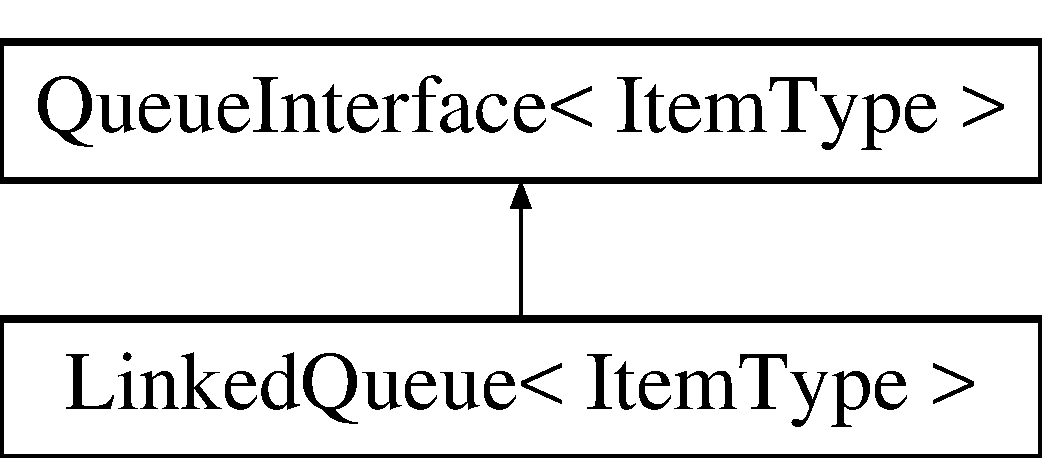
\includegraphics[height=2.000000cm]{class_linked_queue}
\end{center}
\end{figure}
\subsubsection*{Public Member Functions}
\begin{DoxyCompactItemize}
\item 
{\bfseries Linked\+Queue} (const \hyperlink{class_linked_queue}{Linked\+Queue} \&a\+Queue)\hypertarget{class_linked_queue_af17a17a7aa2e191b957d51a73fd54108}{}\label{class_linked_queue_af17a17a7aa2e191b957d51a73fd54108}

\item 
bool \hyperlink{class_linked_queue_ab7c69e207152221746b0d9b089ad4690}{is\+Empty} () const 
\item 
bool \hyperlink{class_linked_queue_a3a46a8aa575cc665f83eae4610837998}{enqueue} (const Item\+Type \&new\+Entry)
\item 
bool \hyperlink{class_linked_queue_a9058a9285a7f8ff6fd27b72347602162}{dequeue} ()
\item 
Item\+Type \hyperlink{class_linked_queue_a712f57ac62e93c0e13af4e0f18aa4fcd}{peek\+Front} () const   throw (\+Precond\+Violated\+Except)
\end{DoxyCompactItemize}


\subsubsection{Member Function Documentation}
\index{Linked\+Queue@{Linked\+Queue}!dequeue@{dequeue}}
\index{dequeue@{dequeue}!Linked\+Queue@{Linked\+Queue}}
\paragraph[{\texorpdfstring{dequeue()}{dequeue()}}]{\setlength{\rightskip}{0pt plus 5cm}template$<$class Item\+Type $>$ bool {\bf Linked\+Queue}$<$ Item\+Type $>$\+::dequeue (
\begin{DoxyParamCaption}
{}
\end{DoxyParamCaption}
)\hspace{0.3cm}{\ttfamily [virtual]}}\hypertarget{class_linked_queue_a9058a9285a7f8ff6fd27b72347602162}{}\label{class_linked_queue_a9058a9285a7f8ff6fd27b72347602162}
Removes the front of this queue. \begin{DoxyPostcond}{Postcondition}
If the operation was successful, the front of the queue has been removed. 
\end{DoxyPostcond}
\begin{DoxyReturn}{Returns}
True if the removal is successful or false if not. 
\end{DoxyReturn}


Implements \hyperlink{class_queue_interface_a0d0d1b1a8b84bee0c3d8c4798a95e792}{Queue\+Interface$<$ Item\+Type $>$}.

\index{Linked\+Queue@{Linked\+Queue}!enqueue@{enqueue}}
\index{enqueue@{enqueue}!Linked\+Queue@{Linked\+Queue}}
\paragraph[{\texorpdfstring{enqueue(const Item\+Type \&new\+Entry)}{enqueue(const ItemType &newEntry)}}]{\setlength{\rightskip}{0pt plus 5cm}template$<$class Item\+Type $>$ bool {\bf Linked\+Queue}$<$ Item\+Type $>$\+::enqueue (
\begin{DoxyParamCaption}
\item[{const Item\+Type \&}]{new\+Entry}
\end{DoxyParamCaption}
)\hspace{0.3cm}{\ttfamily [virtual]}}\hypertarget{class_linked_queue_a3a46a8aa575cc665f83eae4610837998}{}\label{class_linked_queue_a3a46a8aa575cc665f83eae4610837998}
Adds a new entry to the back of this queue. \begin{DoxyPostcond}{Postcondition}
If the operation was successful, new\+Entry is at the back of the queue. 
\end{DoxyPostcond}

\begin{DoxyParams}{Parameters}
{\em new\+Entry} & The object to be added as a new entry. \\
\hline
\end{DoxyParams}
\begin{DoxyReturn}{Returns}
True if the addition is successful or false if not. 
\end{DoxyReturn}


Implements \hyperlink{class_queue_interface_af65d0ec8ce74a1c03ba83ba569cb7c14}{Queue\+Interface$<$ Item\+Type $>$}.

\index{Linked\+Queue@{Linked\+Queue}!is\+Empty@{is\+Empty}}
\index{is\+Empty@{is\+Empty}!Linked\+Queue@{Linked\+Queue}}
\paragraph[{\texorpdfstring{is\+Empty() const }{isEmpty() const }}]{\setlength{\rightskip}{0pt plus 5cm}template$<$class Item\+Type $>$ bool {\bf Linked\+Queue}$<$ Item\+Type $>$\+::is\+Empty (
\begin{DoxyParamCaption}
{}
\end{DoxyParamCaption}
) const\hspace{0.3cm}{\ttfamily [virtual]}}\hypertarget{class_linked_queue_ab7c69e207152221746b0d9b089ad4690}{}\label{class_linked_queue_ab7c69e207152221746b0d9b089ad4690}
Sees whether this queue is empty. \begin{DoxyReturn}{Returns}
True if the queue is empty, or false if not. 
\end{DoxyReturn}


Implements \hyperlink{class_queue_interface_adfc78ad2af130ad5f0867de0e9f63ec7}{Queue\+Interface$<$ Item\+Type $>$}.

\index{Linked\+Queue@{Linked\+Queue}!peek\+Front@{peek\+Front}}
\index{peek\+Front@{peek\+Front}!Linked\+Queue@{Linked\+Queue}}
\paragraph[{\texorpdfstring{peek\+Front() const }{peekFront() const }}]{\setlength{\rightskip}{0pt plus 5cm}template$<$class Item\+Type $>$ Item\+Type {\bf Linked\+Queue}$<$ Item\+Type $>$\+::peek\+Front (
\begin{DoxyParamCaption}
{}
\end{DoxyParamCaption}
) const throw  {\bf Precond\+Violated\+Except}) \hspace{0.3cm}{\ttfamily [virtual]}}\hypertarget{class_linked_queue_a712f57ac62e93c0e13af4e0f18aa4fcd}{}\label{class_linked_queue_a712f57ac62e93c0e13af4e0f18aa4fcd}

\begin{DoxyExceptions}{Exceptions}
{\em \hyperlink{class_precond_violated_except}{Precond\+Violated\+Except}} & if the queue is empty \\
\hline
\end{DoxyExceptions}


Implements \hyperlink{class_queue_interface_a9a6097cc3742158736ef0908586e2066}{Queue\+Interface$<$ Item\+Type $>$}.



The documentation for this class was generated from the following files\+:\begin{DoxyCompactItemize}
\item 
\hyperlink{_linked_queue_8h}{Linked\+Queue.\+h}\item 
Linked\+Queue.\+cpp\end{DoxyCompactItemize}

\hypertarget{class_list_interface}{}\subsection{List\+Interface$<$ Item\+Type $>$ Class Template Reference}
\label{class_list_interface}\index{List\+Interface$<$ Item\+Type $>$@{List\+Interface$<$ Item\+Type $>$}}
Inheritance diagram for List\+Interface$<$ Item\+Type $>$\+:\begin{figure}[H]
\begin{center}
\leavevmode
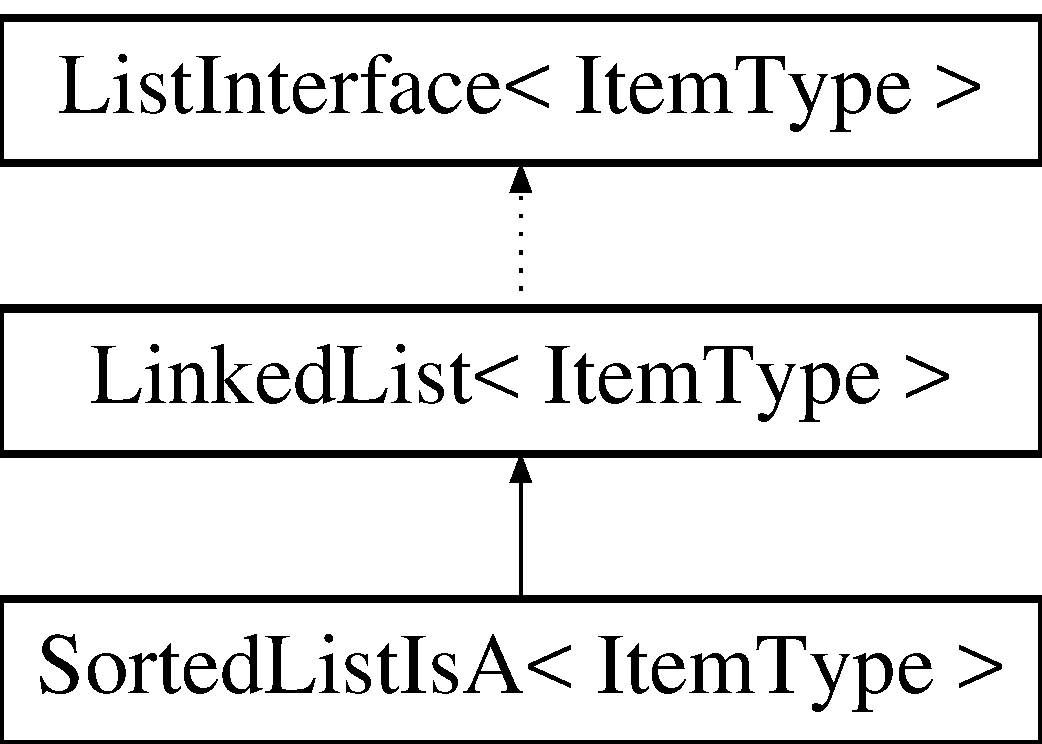
\includegraphics[height=3.000000cm]{class_list_interface}
\end{center}
\end{figure}
\subsubsection*{Public Member Functions}
\begin{DoxyCompactItemize}
\item 
virtual bool \hyperlink{class_list_interface_a924f91e7f81d7dcd3fda79bbcc671394}{is\+Empty} () const =0
\item 
virtual int \hyperlink{class_list_interface_afc85695d4137f1e29ff02e179c9f3221}{get\+Length} () const =0
\item 
virtual bool \hyperlink{class_list_interface_a5b2f86954a86172699a3495982c38e77}{insert} (int new\+Position, const Item\+Type \&new\+Entry)=0
\item 
virtual bool \hyperlink{class_list_interface_a5543002ec0d64bd2a63f3732f437af65}{remove} (int position)=0
\item 
virtual void \hyperlink{class_list_interface_adfda414908b645bdf19bcab8269168b7}{clear} ()=0
\item 
virtual Item\+Type \hyperlink{class_list_interface_a86987f69e5056d287212ede41db1956a}{get\+Entry} (int position) const =0
\item 
virtual void \hyperlink{class_list_interface_aae877a56b7b9f5f526c37a00e234fad1}{replace} (int position, const Item\+Type \&new\+Entry)=0
\end{DoxyCompactItemize}


\subsubsection{Member Function Documentation}
\index{List\+Interface@{List\+Interface}!clear@{clear}}
\index{clear@{clear}!List\+Interface@{List\+Interface}}
\paragraph[{\texorpdfstring{clear()=0}{clear()=0}}]{\setlength{\rightskip}{0pt plus 5cm}template$<$class Item\+Type $>$ virtual void {\bf List\+Interface}$<$ Item\+Type $>$\+::clear (
\begin{DoxyParamCaption}
{}
\end{DoxyParamCaption}
)\hspace{0.3cm}{\ttfamily [pure virtual]}}\hypertarget{class_list_interface_adfda414908b645bdf19bcab8269168b7}{}\label{class_list_interface_adfda414908b645bdf19bcab8269168b7}
Removes all entries from this list. \begin{DoxyPostcond}{Postcondition}
List contains no entries and the count of items is 0. 
\end{DoxyPostcond}


Implemented in \hyperlink{class_linked_list_a7d1d9cf83eef67b6c4d700a3cc5970e1}{Linked\+List$<$ Item\+Type $>$}.

\index{List\+Interface@{List\+Interface}!get\+Entry@{get\+Entry}}
\index{get\+Entry@{get\+Entry}!List\+Interface@{List\+Interface}}
\paragraph[{\texorpdfstring{get\+Entry(int position) const =0}{getEntry(int position) const =0}}]{\setlength{\rightskip}{0pt plus 5cm}template$<$class Item\+Type $>$ virtual Item\+Type {\bf List\+Interface}$<$ Item\+Type $>$\+::get\+Entry (
\begin{DoxyParamCaption}
\item[{int}]{position}
\end{DoxyParamCaption}
) const\hspace{0.3cm}{\ttfamily [pure virtual]}}\hypertarget{class_list_interface_a86987f69e5056d287212ede41db1956a}{}\label{class_list_interface_a86987f69e5056d287212ede41db1956a}
Gets the entry at the given position in this list. \begin{DoxyPrecond}{Precondition}
1 $<$= position $<$= \hyperlink{class_list_interface_afc85695d4137f1e29ff02e179c9f3221}{get\+Length()}. 
\end{DoxyPrecond}
\begin{DoxyPostcond}{Postcondition}
The desired entry has been returned. 
\end{DoxyPostcond}

\begin{DoxyParams}{Parameters}
{\em position} & The list position of the desired entry. \\
\hline
\end{DoxyParams}
\begin{DoxyReturn}{Returns}
The entry at the given position. 
\end{DoxyReturn}


Implemented in \hyperlink{class_linked_list_a79f005e696c19f6ccf90d9d535afa999}{Linked\+List$<$ Item\+Type $>$}.

\index{List\+Interface@{List\+Interface}!get\+Length@{get\+Length}}
\index{get\+Length@{get\+Length}!List\+Interface@{List\+Interface}}
\paragraph[{\texorpdfstring{get\+Length() const =0}{getLength() const =0}}]{\setlength{\rightskip}{0pt plus 5cm}template$<$class Item\+Type $>$ virtual int {\bf List\+Interface}$<$ Item\+Type $>$\+::get\+Length (
\begin{DoxyParamCaption}
{}
\end{DoxyParamCaption}
) const\hspace{0.3cm}{\ttfamily [pure virtual]}}\hypertarget{class_list_interface_afc85695d4137f1e29ff02e179c9f3221}{}\label{class_list_interface_afc85695d4137f1e29ff02e179c9f3221}
Gets the current number of entries in this list. \begin{DoxyReturn}{Returns}
The integer number of entries currently in the list. 
\end{DoxyReturn}


Implemented in \hyperlink{class_linked_list_adae55d6b79235c816cb9e05027fd2e7a}{Linked\+List$<$ Item\+Type $>$}.

\index{List\+Interface@{List\+Interface}!insert@{insert}}
\index{insert@{insert}!List\+Interface@{List\+Interface}}
\paragraph[{\texorpdfstring{insert(int new\+Position, const Item\+Type \&new\+Entry)=0}{insert(int newPosition, const ItemType &newEntry)=0}}]{\setlength{\rightskip}{0pt plus 5cm}template$<$class Item\+Type $>$ virtual bool {\bf List\+Interface}$<$ Item\+Type $>$\+::insert (
\begin{DoxyParamCaption}
\item[{int}]{new\+Position, }
\item[{const Item\+Type \&}]{new\+Entry}
\end{DoxyParamCaption}
)\hspace{0.3cm}{\ttfamily [pure virtual]}}\hypertarget{class_list_interface_a5b2f86954a86172699a3495982c38e77}{}\label{class_list_interface_a5b2f86954a86172699a3495982c38e77}
Inserts an entry into this list at a given position. \begin{DoxyPrecond}{Precondition}
None. 
\end{DoxyPrecond}
\begin{DoxyPostcond}{Postcondition}
If 1 $<$= position $<$= \hyperlink{class_list_interface_afc85695d4137f1e29ff02e179c9f3221}{get\+Length()} + 1 and the insertion is successful, new\+Entry is at the given position in the list, other entries are renumbered accordingly, and the returned value is true. 
\end{DoxyPostcond}

\begin{DoxyParams}{Parameters}
{\em new\+Position} & The list position at which to insert new\+Entry. \\
\hline
{\em new\+Entry} & The entry to insert into the list. \\
\hline
\end{DoxyParams}
\begin{DoxyReturn}{Returns}
True if insertion is successful, or false if not. 
\end{DoxyReturn}


Implemented in \hyperlink{class_linked_list_ae8a19375505e87e2e4fc0e9b5afe4d4d}{Linked\+List$<$ Item\+Type $>$}, and \hyperlink{class_sorted_list_is_a_aa80ef5215183e3a17f2a2f2e76d4fca3}{Sorted\+List\+Is\+A$<$ Item\+Type $>$}.

\index{List\+Interface@{List\+Interface}!is\+Empty@{is\+Empty}}
\index{is\+Empty@{is\+Empty}!List\+Interface@{List\+Interface}}
\paragraph[{\texorpdfstring{is\+Empty() const =0}{isEmpty() const =0}}]{\setlength{\rightskip}{0pt plus 5cm}template$<$class Item\+Type $>$ virtual bool {\bf List\+Interface}$<$ Item\+Type $>$\+::is\+Empty (
\begin{DoxyParamCaption}
{}
\end{DoxyParamCaption}
) const\hspace{0.3cm}{\ttfamily [pure virtual]}}\hypertarget{class_list_interface_a924f91e7f81d7dcd3fda79bbcc671394}{}\label{class_list_interface_a924f91e7f81d7dcd3fda79bbcc671394}
Sees whether this list is empty. \begin{DoxyReturn}{Returns}
True if the list is empty; otherwise returns false. 
\end{DoxyReturn}


Implemented in \hyperlink{class_linked_list_adb17aed0ceacbbe1f247d235f491f0d5}{Linked\+List$<$ Item\+Type $>$}.

\index{List\+Interface@{List\+Interface}!remove@{remove}}
\index{remove@{remove}!List\+Interface@{List\+Interface}}
\paragraph[{\texorpdfstring{remove(int position)=0}{remove(int position)=0}}]{\setlength{\rightskip}{0pt plus 5cm}template$<$class Item\+Type $>$ virtual bool {\bf List\+Interface}$<$ Item\+Type $>$\+::remove (
\begin{DoxyParamCaption}
\item[{int}]{position}
\end{DoxyParamCaption}
)\hspace{0.3cm}{\ttfamily [pure virtual]}}\hypertarget{class_list_interface_a5543002ec0d64bd2a63f3732f437af65}{}\label{class_list_interface_a5543002ec0d64bd2a63f3732f437af65}
Removes the entry at a given position from this list. \begin{DoxyPrecond}{Precondition}
None. 
\end{DoxyPrecond}
\begin{DoxyPostcond}{Postcondition}
If 1 $<$= position $<$= \hyperlink{class_list_interface_afc85695d4137f1e29ff02e179c9f3221}{get\+Length()} and the removal is successful, the entry at the given position in the list is removed, other items are renumbered accordingly, and the returned value is true. 
\end{DoxyPostcond}

\begin{DoxyParams}{Parameters}
{\em position} & The list position of the entry to remove. \\
\hline
\end{DoxyParams}
\begin{DoxyReturn}{Returns}
True if removal is successful, or false if not. 
\end{DoxyReturn}


Implemented in \hyperlink{class_linked_list_a16a02716b5b2efb6fb1e3d18721b53e4}{Linked\+List$<$ Item\+Type $>$}.

\index{List\+Interface@{List\+Interface}!replace@{replace}}
\index{replace@{replace}!List\+Interface@{List\+Interface}}
\paragraph[{\texorpdfstring{replace(int position, const Item\+Type \&new\+Entry)=0}{replace(int position, const ItemType &newEntry)=0}}]{\setlength{\rightskip}{0pt plus 5cm}template$<$class Item\+Type $>$ virtual void {\bf List\+Interface}$<$ Item\+Type $>$\+::replace (
\begin{DoxyParamCaption}
\item[{int}]{position, }
\item[{const Item\+Type \&}]{new\+Entry}
\end{DoxyParamCaption}
)\hspace{0.3cm}{\ttfamily [pure virtual]}}\hypertarget{class_list_interface_aae877a56b7b9f5f526c37a00e234fad1}{}\label{class_list_interface_aae877a56b7b9f5f526c37a00e234fad1}
Replaces the entry at the given position in this list. \begin{DoxyPrecond}{Precondition}
1 $<$= position $<$= \hyperlink{class_list_interface_afc85695d4137f1e29ff02e179c9f3221}{get\+Length()}. 
\end{DoxyPrecond}
\begin{DoxyPostcond}{Postcondition}
The entry at the given position is new\+Entry. 
\end{DoxyPostcond}

\begin{DoxyParams}{Parameters}
{\em position} & The list position of the entry to replace. \\
\hline
{\em new\+Entry} & The replacement entry. \\
\hline
\end{DoxyParams}


Implemented in \hyperlink{class_linked_list_a3035f880c50e7d8f68e67c093d4607ca}{Linked\+List$<$ Item\+Type $>$}, and \hyperlink{class_sorted_list_is_a_ae85cca0f8a4a306d6d28cc5993e5895c}{Sorted\+List\+Is\+A$<$ Item\+Type $>$}.



The documentation for this class was generated from the following file\+:\begin{DoxyCompactItemize}
\item 
\hyperlink{_list_interface_8h}{List\+Interface.\+h}\end{DoxyCompactItemize}

\hypertarget{class_node}{\subsection{Node$<$ Item\-Type $>$ Class Template Reference}
\label{class_node}\index{Node$<$ Item\-Type $>$@{Node$<$ Item\-Type $>$}}
}
\subsubsection*{Public Member Functions}
\begin{DoxyCompactItemize}
\item 
\hyperlink{class_node_a627e94f4fba0e73c546e0fb2a7266f36}{Node} ()
\item 
\hyperlink{class_node_a0288598fcb0244739ce95099c26250ae}{Node} (const Item\-Type \&an\-Item)
\item 
\hyperlink{class_node_adf98d3f9b7227622cb5a0fdd7e8f0b18}{Node} (const Item\-Type \&an\-Item, \hyperlink{class_node}{Node}$<$ Item\-Type $>$ $\ast$next\-Node\-Ptr)
\item 
void \hyperlink{class_node_ab4ceecdecc5df799011de486b9f54974}{set\-Item} (const Item\-Type \&an\-Item)
\item 
void \hyperlink{class_node_a01c1a66d4e39f5b149e090413deb4633}{set\-Next} (\hyperlink{class_node}{Node}$<$ Item\-Type $>$ $\ast$next\-Node\-Ptr)
\item 
Item\-Type \hyperlink{class_node_a4e5519463291a0c1570014f4ee5ca130}{get\-Item} () const 
\item 
\hyperlink{class_node}{Node}$<$ Item\-Type $>$ $\ast$ \hyperlink{class_node_a44fbda8e8d17a37e8203434c2909ea07}{get\-Next} () const 
\end{DoxyCompactItemize}
\subsubsection*{Private Attributes}
\begin{DoxyCompactItemize}
\item 
\hypertarget{class_node_a73e84414314067aa019ba6afb06190bd}{Item\-Type {\bfseries item}}\label{class_node_a73e84414314067aa019ba6afb06190bd}

\item 
\hypertarget{class_node_ad11288556b42a32b4f46ed955b7c31fd}{\hyperlink{class_node}{Node}$<$ Item\-Type $>$ $\ast$ {\bfseries next}}\label{class_node_ad11288556b42a32b4f46ed955b7c31fd}

\end{DoxyCompactItemize}


\subsubsection{Constructor \& Destructor Documentation}
\hypertarget{class_node_a627e94f4fba0e73c546e0fb2a7266f36}{\index{Node@{Node}!Node@{Node}}
\index{Node@{Node}!Node@{Node}}
\paragraph[{Node}]{\setlength{\rightskip}{0pt plus 5cm}template$<$class Item\-Type $>$ {\bf Node}$<$ Item\-Type $>$\-::{\bf Node} (
\begin{DoxyParamCaption}
{}
\end{DoxyParamCaption}
)}}\label{class_node_a627e94f4fba0e73c546e0fb2a7266f36}
default constructor \hypertarget{class_node_a0288598fcb0244739ce95099c26250ae}{\index{Node@{Node}!Node@{Node}}
\index{Node@{Node}!Node@{Node}}
\paragraph[{Node}]{\setlength{\rightskip}{0pt plus 5cm}template$<$class Item\-Type $>$ {\bf Node}$<$ Item\-Type $>$\-::{\bf Node} (
\begin{DoxyParamCaption}
\item[{const Item\-Type \&}]{an\-Item}
\end{DoxyParamCaption}
)}}\label{class_node_a0288598fcb0244739ce95099c26250ae}
constructor with item value \hypertarget{class_node_adf98d3f9b7227622cb5a0fdd7e8f0b18}{\index{Node@{Node}!Node@{Node}}
\index{Node@{Node}!Node@{Node}}
\paragraph[{Node}]{\setlength{\rightskip}{0pt plus 5cm}template$<$class Item\-Type $>$ {\bf Node}$<$ Item\-Type $>$\-::{\bf Node} (
\begin{DoxyParamCaption}
\item[{const Item\-Type \&}]{an\-Item, }
\item[{{\bf Node}$<$ Item\-Type $>$ $\ast$}]{next\-Node\-Ptr}
\end{DoxyParamCaption}
)}}\label{class_node_adf98d3f9b7227622cb5a0fdd7e8f0b18}
constructor with item value and next pointer 

\subsubsection{Member Function Documentation}
\hypertarget{class_node_a4e5519463291a0c1570014f4ee5ca130}{\index{Node@{Node}!get\-Item@{get\-Item}}
\index{get\-Item@{get\-Item}!Node@{Node}}
\paragraph[{get\-Item}]{\setlength{\rightskip}{0pt plus 5cm}template$<$class Item\-Type $>$ Item\-Type {\bf Node}$<$ Item\-Type $>$\-::get\-Item (
\begin{DoxyParamCaption}
{}
\end{DoxyParamCaption}
) const}}\label{class_node_a4e5519463291a0c1570014f4ee5ca130}
returns the item stored in the node \hypertarget{class_node_a44fbda8e8d17a37e8203434c2909ea07}{\index{Node@{Node}!get\-Next@{get\-Next}}
\index{get\-Next@{get\-Next}!Node@{Node}}
\paragraph[{get\-Next}]{\setlength{\rightskip}{0pt plus 5cm}template$<$class Item\-Type $>$ {\bf Node}$<$ Item\-Type $>$ $\ast$ {\bf Node}$<$ Item\-Type $>$\-::get\-Next (
\begin{DoxyParamCaption}
{}
\end{DoxyParamCaption}
) const}}\label{class_node_a44fbda8e8d17a37e8203434c2909ea07}
returns the next node \hypertarget{class_node_ab4ceecdecc5df799011de486b9f54974}{\index{Node@{Node}!set\-Item@{set\-Item}}
\index{set\-Item@{set\-Item}!Node@{Node}}
\paragraph[{set\-Item}]{\setlength{\rightskip}{0pt plus 5cm}template$<$class Item\-Type $>$ void {\bf Node}$<$ Item\-Type $>$\-::set\-Item (
\begin{DoxyParamCaption}
\item[{const Item\-Type \&}]{an\-Item}
\end{DoxyParamCaption}
)}}\label{class_node_ab4ceecdecc5df799011de486b9f54974}
sets the item value of the node \hypertarget{class_node_a01c1a66d4e39f5b149e090413deb4633}{\index{Node@{Node}!set\-Next@{set\-Next}}
\index{set\-Next@{set\-Next}!Node@{Node}}
\paragraph[{set\-Next}]{\setlength{\rightskip}{0pt plus 5cm}template$<$class Item\-Type $>$ void {\bf Node}$<$ Item\-Type $>$\-::set\-Next (
\begin{DoxyParamCaption}
\item[{{\bf Node}$<$ Item\-Type $>$ $\ast$}]{next\-Node\-Ptr}
\end{DoxyParamCaption}
)}}\label{class_node_a01c1a66d4e39f5b149e090413deb4633}
sets the pointer to the next node 

The documentation for this class was generated from the following files\-:\begin{DoxyCompactItemize}
\item 
\hyperlink{_node_8h}{Node.\-h}\item 
\hyperlink{_node_8cpp}{Node.\-cpp}\end{DoxyCompactItemize}

\hypertarget{class_precond_violated_except}{\subsection{Precond\-Violated\-Except Class Reference}
\label{class_precond_violated_except}\index{Precond\-Violated\-Except@{Precond\-Violated\-Except}}
}
Inheritance diagram for Precond\-Violated\-Except\-:\begin{figure}[H]
\begin{center}
\leavevmode
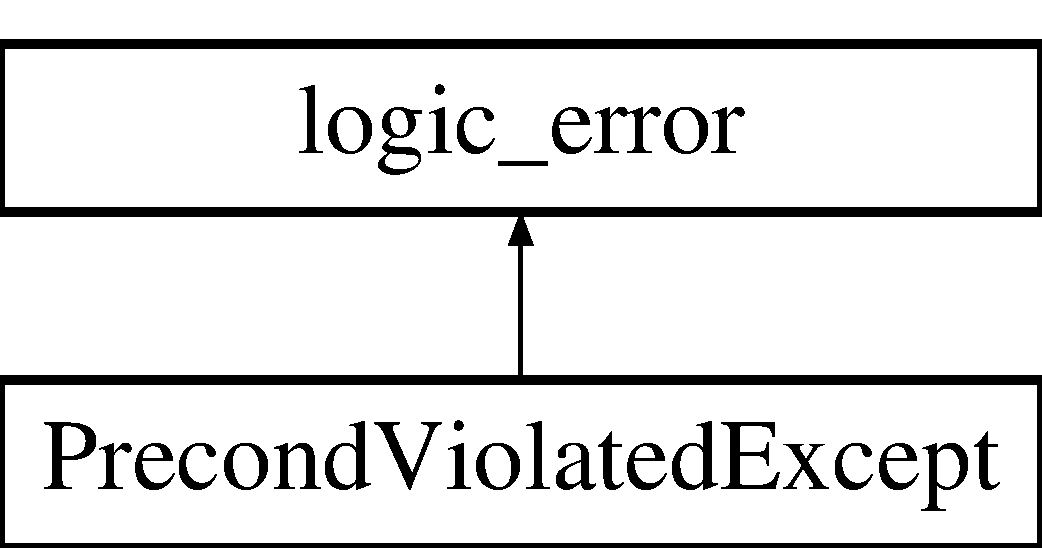
\includegraphics[height=2.000000cm]{class_precond_violated_except}
\end{center}
\end{figure}
\subsubsection*{Public Member Functions}
\begin{DoxyCompactItemize}
\item 
\hypertarget{class_precond_violated_except_a13c9075198f291ffc9a74c0c9b787ecf}{{\bfseries Precond\-Violated\-Except} (const std\-::string \&message=\char`\"{}\char`\"{})}\label{class_precond_violated_except_a13c9075198f291ffc9a74c0c9b787ecf}

\end{DoxyCompactItemize}


The documentation for this class was generated from the following files\-:\begin{DoxyCompactItemize}
\item 
\hyperlink{_precond_violated_except_8h}{Precond\-Violated\-Except.\-h}\item 
\hyperlink{_precond_violated_except_8cpp}{Precond\-Violated\-Except.\-cpp}\end{DoxyCompactItemize}

\hypertarget{class_priority_queue_interface}{}\subsection{Priority\+Queue\+Interface$<$ Item\+Type $>$ Class Template Reference}
\label{class_priority_queue_interface}\index{Priority\+Queue\+Interface$<$ Item\+Type $>$@{Priority\+Queue\+Interface$<$ Item\+Type $>$}}
Inheritance diagram for Priority\+Queue\+Interface$<$ Item\+Type $>$\+:\begin{figure}[H]
\begin{center}
\leavevmode
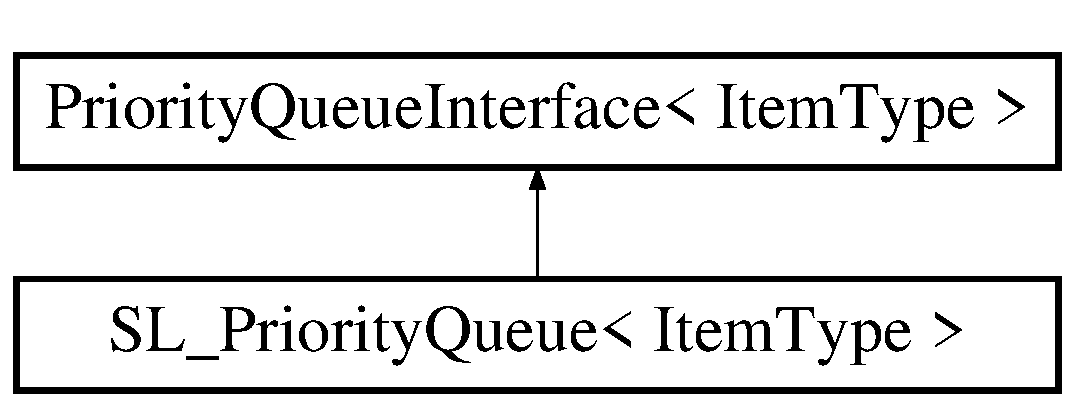
\includegraphics[height=2.000000cm]{class_priority_queue_interface}
\end{center}
\end{figure}
\subsubsection*{Public Member Functions}
\begin{DoxyCompactItemize}
\item 
virtual bool \hyperlink{class_priority_queue_interface_ad3f9d9c3dc7bc50ca9cbf3d4ec243608}{is\+Empty} () const =0
\item 
virtual bool \hyperlink{class_priority_queue_interface_ab45542786f10cf88ec8c7d05fba96124}{enqueue} (const Item\+Type \&new\+Entry)=0
\item 
virtual bool \hyperlink{class_priority_queue_interface_abc4b28c8515af5b648c86e7a1af01ae9}{dequeue} ()=0
\item 
virtual Item\+Type \hyperlink{class_priority_queue_interface_aa0e45d144ef82101311ab83501dd403b}{peek\+Front} () const =0
\item 
virtual \hyperlink{class_priority_queue_interface_a4fc01b49a8e0799b86a3c5ba25910470}{$\sim$\+Priority\+Queue\+Interface} ()
\end{DoxyCompactItemize}


\subsubsection{Constructor \& Destructor Documentation}
\index{Priority\+Queue\+Interface@{Priority\+Queue\+Interface}!````~Priority\+Queue\+Interface@{$\sim$\+Priority\+Queue\+Interface}}
\index{````~Priority\+Queue\+Interface@{$\sim$\+Priority\+Queue\+Interface}!Priority\+Queue\+Interface@{Priority\+Queue\+Interface}}
\paragraph[{\texorpdfstring{$\sim$\+Priority\+Queue\+Interface()}{~PriorityQueueInterface()}}]{\setlength{\rightskip}{0pt plus 5cm}template$<$class Item\+Type $>$ virtual {\bf Priority\+Queue\+Interface}$<$ Item\+Type $>$\+::$\sim${\bf Priority\+Queue\+Interface} (
\begin{DoxyParamCaption}
{}
\end{DoxyParamCaption}
)\hspace{0.3cm}{\ttfamily [inline]}, {\ttfamily [virtual]}}\hypertarget{class_priority_queue_interface_a4fc01b49a8e0799b86a3c5ba25910470}{}\label{class_priority_queue_interface_a4fc01b49a8e0799b86a3c5ba25910470}
Destroys this queue and frees its memory. 

\subsubsection{Member Function Documentation}
\index{Priority\+Queue\+Interface@{Priority\+Queue\+Interface}!dequeue@{dequeue}}
\index{dequeue@{dequeue}!Priority\+Queue\+Interface@{Priority\+Queue\+Interface}}
\paragraph[{\texorpdfstring{dequeue()=0}{dequeue()=0}}]{\setlength{\rightskip}{0pt plus 5cm}template$<$class Item\+Type $>$ virtual bool {\bf Priority\+Queue\+Interface}$<$ Item\+Type $>$\+::dequeue (
\begin{DoxyParamCaption}
{}
\end{DoxyParamCaption}
)\hspace{0.3cm}{\ttfamily [pure virtual]}}\hypertarget{class_priority_queue_interface_abc4b28c8515af5b648c86e7a1af01ae9}{}\label{class_priority_queue_interface_abc4b28c8515af5b648c86e7a1af01ae9}
Removes the front of this queue. \begin{DoxyPostcond}{Postcondition}
If the operation was successful, the front of the queue has been removed. 
\end{DoxyPostcond}
\begin{DoxyReturn}{Returns}
True if the removal is successful or false if not. 
\end{DoxyReturn}


Implemented in \hyperlink{class_s_l___priority_queue_ac9ec261fab4c5834c5e9d1aeb15833c7}{S\+L\+\_\+\+Priority\+Queue$<$ Item\+Type $>$}.

\index{Priority\+Queue\+Interface@{Priority\+Queue\+Interface}!enqueue@{enqueue}}
\index{enqueue@{enqueue}!Priority\+Queue\+Interface@{Priority\+Queue\+Interface}}
\paragraph[{\texorpdfstring{enqueue(const Item\+Type \&new\+Entry)=0}{enqueue(const ItemType &newEntry)=0}}]{\setlength{\rightskip}{0pt plus 5cm}template$<$class Item\+Type $>$ virtual bool {\bf Priority\+Queue\+Interface}$<$ Item\+Type $>$\+::enqueue (
\begin{DoxyParamCaption}
\item[{const Item\+Type \&}]{new\+Entry}
\end{DoxyParamCaption}
)\hspace{0.3cm}{\ttfamily [pure virtual]}}\hypertarget{class_priority_queue_interface_ab45542786f10cf88ec8c7d05fba96124}{}\label{class_priority_queue_interface_ab45542786f10cf88ec8c7d05fba96124}
Adds a new entry to the back of this queue. \begin{DoxyPostcond}{Postcondition}
If the operation was successful, new\+Entry is at the back of the queue. 
\end{DoxyPostcond}

\begin{DoxyParams}{Parameters}
{\em new\+Entry} & The object to be added as a new entry. \\
\hline
\end{DoxyParams}
\begin{DoxyReturn}{Returns}
True if the addition is successful or false if not. 
\end{DoxyReturn}


Implemented in \hyperlink{class_s_l___priority_queue_a23d14a8e92ba404f771eb5e99aee3c77}{S\+L\+\_\+\+Priority\+Queue$<$ Item\+Type $>$}.

\index{Priority\+Queue\+Interface@{Priority\+Queue\+Interface}!is\+Empty@{is\+Empty}}
\index{is\+Empty@{is\+Empty}!Priority\+Queue\+Interface@{Priority\+Queue\+Interface}}
\paragraph[{\texorpdfstring{is\+Empty() const =0}{isEmpty() const =0}}]{\setlength{\rightskip}{0pt plus 5cm}template$<$class Item\+Type $>$ virtual bool {\bf Priority\+Queue\+Interface}$<$ Item\+Type $>$\+::is\+Empty (
\begin{DoxyParamCaption}
{}
\end{DoxyParamCaption}
) const\hspace{0.3cm}{\ttfamily [pure virtual]}}\hypertarget{class_priority_queue_interface_ad3f9d9c3dc7bc50ca9cbf3d4ec243608}{}\label{class_priority_queue_interface_ad3f9d9c3dc7bc50ca9cbf3d4ec243608}
Sees whether this queue is empty. \begin{DoxyReturn}{Returns}
True if the queue is empty, or false if not. 
\end{DoxyReturn}


Implemented in \hyperlink{class_s_l___priority_queue_a4502c0091ed41cbedc3fb25040ae2833}{S\+L\+\_\+\+Priority\+Queue$<$ Item\+Type $>$}.

\index{Priority\+Queue\+Interface@{Priority\+Queue\+Interface}!peek\+Front@{peek\+Front}}
\index{peek\+Front@{peek\+Front}!Priority\+Queue\+Interface@{Priority\+Queue\+Interface}}
\paragraph[{\texorpdfstring{peek\+Front() const =0}{peekFront() const =0}}]{\setlength{\rightskip}{0pt plus 5cm}template$<$class Item\+Type $>$ virtual Item\+Type {\bf Priority\+Queue\+Interface}$<$ Item\+Type $>$\+::peek\+Front (
\begin{DoxyParamCaption}
{}
\end{DoxyParamCaption}
) const\hspace{0.3cm}{\ttfamily [pure virtual]}}\hypertarget{class_priority_queue_interface_aa0e45d144ef82101311ab83501dd403b}{}\label{class_priority_queue_interface_aa0e45d144ef82101311ab83501dd403b}
Returns the front of this queue. \begin{DoxyPrecond}{Precondition}
The queue is not empty. 
\end{DoxyPrecond}
\begin{DoxyPostcond}{Postcondition}
The front of the queue has been returned, and the queue is unchanged. 
\end{DoxyPostcond}
\begin{DoxyReturn}{Returns}
The front of the queue. 
\end{DoxyReturn}


Implemented in \hyperlink{class_s_l___priority_queue_ade728bc676a9f65ab8cf70b4f498afa3}{S\+L\+\_\+\+Priority\+Queue$<$ Item\+Type $>$}.



The documentation for this class was generated from the following file\+:\begin{DoxyCompactItemize}
\item 
\hyperlink{_priority_queue_interface_8h}{Priority\+Queue\+Interface.\+h}\end{DoxyCompactItemize}

\hypertarget{class_queue_interface}{}\subsection{Queue\+Interface$<$ Item\+Type $>$ Class Template Reference}
\label{class_queue_interface}\index{Queue\+Interface$<$ Item\+Type $>$@{Queue\+Interface$<$ Item\+Type $>$}}
Inheritance diagram for Queue\+Interface$<$ Item\+Type $>$\+:\begin{figure}[H]
\begin{center}
\leavevmode
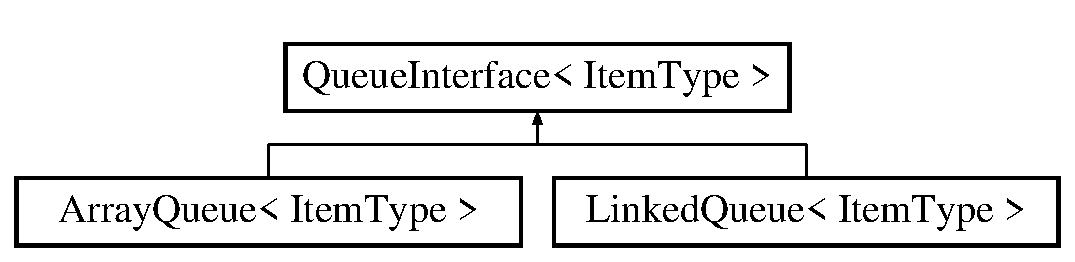
\includegraphics[height=2.000000cm]{class_queue_interface}
\end{center}
\end{figure}
\subsubsection*{Public Member Functions}
\begin{DoxyCompactItemize}
\item 
virtual bool \hyperlink{class_queue_interface_adfc78ad2af130ad5f0867de0e9f63ec7}{is\+Empty} () const =0
\item 
virtual bool \hyperlink{class_queue_interface_af65d0ec8ce74a1c03ba83ba569cb7c14}{enqueue} (const Item\+Type \&new\+Entry)=0
\item 
virtual bool \hyperlink{class_queue_interface_a0d0d1b1a8b84bee0c3d8c4798a95e792}{dequeue} ()=0
\item 
virtual Item\+Type \hyperlink{class_queue_interface_a9a6097cc3742158736ef0908586e2066}{peek\+Front} () const =0
\item 
virtual \hyperlink{class_queue_interface_a35146beb6f3c60972ae75e1d0091e2eb}{$\sim$\+Queue\+Interface} ()
\end{DoxyCompactItemize}


\subsubsection{Constructor \& Destructor Documentation}
\index{Queue\+Interface@{Queue\+Interface}!````~Queue\+Interface@{$\sim$\+Queue\+Interface}}
\index{````~Queue\+Interface@{$\sim$\+Queue\+Interface}!Queue\+Interface@{Queue\+Interface}}
\paragraph[{\texorpdfstring{$\sim$\+Queue\+Interface()}{~QueueInterface()}}]{\setlength{\rightskip}{0pt plus 5cm}template$<$class Item\+Type $>$ virtual {\bf Queue\+Interface}$<$ Item\+Type $>$\+::$\sim${\bf Queue\+Interface} (
\begin{DoxyParamCaption}
{}
\end{DoxyParamCaption}
)\hspace{0.3cm}{\ttfamily [inline]}, {\ttfamily [virtual]}}\hypertarget{class_queue_interface_a35146beb6f3c60972ae75e1d0091e2eb}{}\label{class_queue_interface_a35146beb6f3c60972ae75e1d0091e2eb}
Destroys this queue and frees its memory. 

\subsubsection{Member Function Documentation}
\index{Queue\+Interface@{Queue\+Interface}!dequeue@{dequeue}}
\index{dequeue@{dequeue}!Queue\+Interface@{Queue\+Interface}}
\paragraph[{\texorpdfstring{dequeue()=0}{dequeue()=0}}]{\setlength{\rightskip}{0pt plus 5cm}template$<$class Item\+Type $>$ virtual bool {\bf Queue\+Interface}$<$ Item\+Type $>$\+::dequeue (
\begin{DoxyParamCaption}
{}
\end{DoxyParamCaption}
)\hspace{0.3cm}{\ttfamily [pure virtual]}}\hypertarget{class_queue_interface_a0d0d1b1a8b84bee0c3d8c4798a95e792}{}\label{class_queue_interface_a0d0d1b1a8b84bee0c3d8c4798a95e792}
Removes the front of this queue. \begin{DoxyPostcond}{Postcondition}
If the operation was successful, the front of the queue has been removed. 
\end{DoxyPostcond}
\begin{DoxyReturn}{Returns}
True if the removal is successful or false if not. 
\end{DoxyReturn}


Implemented in \hyperlink{class_linked_queue_a9058a9285a7f8ff6fd27b72347602162}{Linked\+Queue$<$ Item\+Type $>$}, and \hyperlink{class_array_queue_a13a06eec37f359d07a785f831e1f287c}{Array\+Queue$<$ Item\+Type $>$}.

\index{Queue\+Interface@{Queue\+Interface}!enqueue@{enqueue}}
\index{enqueue@{enqueue}!Queue\+Interface@{Queue\+Interface}}
\paragraph[{\texorpdfstring{enqueue(const Item\+Type \&new\+Entry)=0}{enqueue(const ItemType &newEntry)=0}}]{\setlength{\rightskip}{0pt plus 5cm}template$<$class Item\+Type $>$ virtual bool {\bf Queue\+Interface}$<$ Item\+Type $>$\+::enqueue (
\begin{DoxyParamCaption}
\item[{const Item\+Type \&}]{new\+Entry}
\end{DoxyParamCaption}
)\hspace{0.3cm}{\ttfamily [pure virtual]}}\hypertarget{class_queue_interface_af65d0ec8ce74a1c03ba83ba569cb7c14}{}\label{class_queue_interface_af65d0ec8ce74a1c03ba83ba569cb7c14}
Adds a new entry to the back of this queue. \begin{DoxyPostcond}{Postcondition}
If the operation was successful, new\+Entry is at the back of the queue. 
\end{DoxyPostcond}

\begin{DoxyParams}{Parameters}
{\em new\+Entry} & The object to be added as a new entry. \\
\hline
\end{DoxyParams}
\begin{DoxyReturn}{Returns}
True if the addition is successful or false if not. 
\end{DoxyReturn}


Implemented in \hyperlink{class_linked_queue_a3a46a8aa575cc665f83eae4610837998}{Linked\+Queue$<$ Item\+Type $>$}, and \hyperlink{class_array_queue_ae8942e3f72dbbfba821e8d7dabf9ec33}{Array\+Queue$<$ Item\+Type $>$}.

\index{Queue\+Interface@{Queue\+Interface}!is\+Empty@{is\+Empty}}
\index{is\+Empty@{is\+Empty}!Queue\+Interface@{Queue\+Interface}}
\paragraph[{\texorpdfstring{is\+Empty() const =0}{isEmpty() const =0}}]{\setlength{\rightskip}{0pt plus 5cm}template$<$class Item\+Type $>$ virtual bool {\bf Queue\+Interface}$<$ Item\+Type $>$\+::is\+Empty (
\begin{DoxyParamCaption}
{}
\end{DoxyParamCaption}
) const\hspace{0.3cm}{\ttfamily [pure virtual]}}\hypertarget{class_queue_interface_adfc78ad2af130ad5f0867de0e9f63ec7}{}\label{class_queue_interface_adfc78ad2af130ad5f0867de0e9f63ec7}
Sees whether this queue is empty. \begin{DoxyReturn}{Returns}
True if the queue is empty, or false if not. 
\end{DoxyReturn}


Implemented in \hyperlink{class_linked_queue_ab7c69e207152221746b0d9b089ad4690}{Linked\+Queue$<$ Item\+Type $>$}, and \hyperlink{class_array_queue_a9ecf3552d6b73c51f6b81277c6ba453d}{Array\+Queue$<$ Item\+Type $>$}.

\index{Queue\+Interface@{Queue\+Interface}!peek\+Front@{peek\+Front}}
\index{peek\+Front@{peek\+Front}!Queue\+Interface@{Queue\+Interface}}
\paragraph[{\texorpdfstring{peek\+Front() const =0}{peekFront() const =0}}]{\setlength{\rightskip}{0pt plus 5cm}template$<$class Item\+Type $>$ virtual Item\+Type {\bf Queue\+Interface}$<$ Item\+Type $>$\+::peek\+Front (
\begin{DoxyParamCaption}
{}
\end{DoxyParamCaption}
) const\hspace{0.3cm}{\ttfamily [pure virtual]}}\hypertarget{class_queue_interface_a9a6097cc3742158736ef0908586e2066}{}\label{class_queue_interface_a9a6097cc3742158736ef0908586e2066}
Returns the front of this queue. \begin{DoxyPrecond}{Precondition}
The queue is not empty. 
\end{DoxyPrecond}
\begin{DoxyPostcond}{Postcondition}
The front of the queue has been returned, and the queue is unchanged. 
\end{DoxyPostcond}
\begin{DoxyReturn}{Returns}
The front of the queue. 
\end{DoxyReturn}


Implemented in \hyperlink{class_linked_queue_a712f57ac62e93c0e13af4e0f18aa4fcd}{Linked\+Queue$<$ Item\+Type $>$}, and \hyperlink{class_array_queue_aba429775b7eedf84920bb00e78022d8a}{Array\+Queue$<$ Item\+Type $>$}.



The documentation for this class was generated from the following file\+:\begin{DoxyCompactItemize}
\item 
\hyperlink{_queue_interface_8h}{Queue\+Interface.\+h}\end{DoxyCompactItemize}

\hypertarget{class_s_l___priority_queue}{}\subsection{S\+L\+\_\+\+Priority\+Queue$<$ Item\+Type $>$ Class Template Reference}
\label{class_s_l___priority_queue}\index{S\+L\+\_\+\+Priority\+Queue$<$ Item\+Type $>$@{S\+L\+\_\+\+Priority\+Queue$<$ Item\+Type $>$}}
Inheritance diagram for S\+L\+\_\+\+Priority\+Queue$<$ Item\+Type $>$\+:\begin{figure}[H]
\begin{center}
\leavevmode
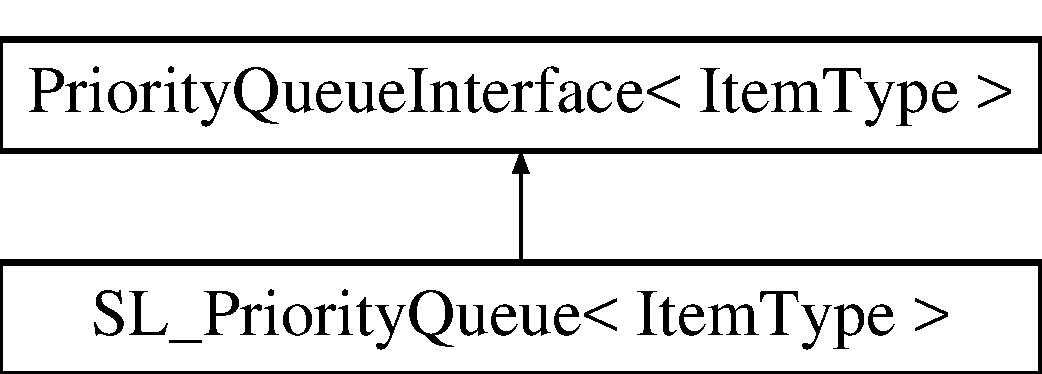
\includegraphics[height=2.000000cm]{class_s_l___priority_queue}
\end{center}
\end{figure}
\subsubsection*{Public Member Functions}
\begin{DoxyCompactItemize}
\item 
{\bfseries S\+L\+\_\+\+Priority\+Queue} (const \hyperlink{class_s_l___priority_queue}{S\+L\+\_\+\+Priority\+Queue} \&pq)\hypertarget{class_s_l___priority_queue_a2630a64cbd7376864bcd4fac9c65991e}{}\label{class_s_l___priority_queue_a2630a64cbd7376864bcd4fac9c65991e}

\item 
bool \hyperlink{class_s_l___priority_queue_a4502c0091ed41cbedc3fb25040ae2833}{is\+Empty} () const 
\item 
bool \hyperlink{class_s_l___priority_queue_a23d14a8e92ba404f771eb5e99aee3c77}{enqueue} (const Item\+Type \&new\+Entry)
\item 
bool \hyperlink{class_s_l___priority_queue_ac9ec261fab4c5834c5e9d1aeb15833c7}{dequeue} ()
\item 
Item\+Type \hyperlink{class_s_l___priority_queue_ade728bc676a9f65ab8cf70b4f498afa3}{peek\+Front} () const   throw (\+Precond\+Violated\+Except)
\end{DoxyCompactItemize}


\subsubsection{Member Function Documentation}
\index{S\+L\+\_\+\+Priority\+Queue@{S\+L\+\_\+\+Priority\+Queue}!dequeue@{dequeue}}
\index{dequeue@{dequeue}!S\+L\+\_\+\+Priority\+Queue@{S\+L\+\_\+\+Priority\+Queue}}
\paragraph[{\texorpdfstring{dequeue()}{dequeue()}}]{\setlength{\rightskip}{0pt plus 5cm}template$<$class Item\+Type $>$ bool {\bf S\+L\+\_\+\+Priority\+Queue}$<$ Item\+Type $>$\+::dequeue (
\begin{DoxyParamCaption}
{}
\end{DoxyParamCaption}
)\hspace{0.3cm}{\ttfamily [virtual]}}\hypertarget{class_s_l___priority_queue_ac9ec261fab4c5834c5e9d1aeb15833c7}{}\label{class_s_l___priority_queue_ac9ec261fab4c5834c5e9d1aeb15833c7}
Removes the front of this queue. \begin{DoxyPostcond}{Postcondition}
If the operation was successful, the front of the queue has been removed. 
\end{DoxyPostcond}
\begin{DoxyReturn}{Returns}
True if the removal is successful or false if not. 
\end{DoxyReturn}


Implements \hyperlink{class_priority_queue_interface_abc4b28c8515af5b648c86e7a1af01ae9}{Priority\+Queue\+Interface$<$ Item\+Type $>$}.

\index{S\+L\+\_\+\+Priority\+Queue@{S\+L\+\_\+\+Priority\+Queue}!enqueue@{enqueue}}
\index{enqueue@{enqueue}!S\+L\+\_\+\+Priority\+Queue@{S\+L\+\_\+\+Priority\+Queue}}
\paragraph[{\texorpdfstring{enqueue(const Item\+Type \&new\+Entry)}{enqueue(const ItemType &newEntry)}}]{\setlength{\rightskip}{0pt plus 5cm}template$<$class Item\+Type $>$ bool {\bf S\+L\+\_\+\+Priority\+Queue}$<$ Item\+Type $>$\+::enqueue (
\begin{DoxyParamCaption}
\item[{const Item\+Type \&}]{new\+Entry}
\end{DoxyParamCaption}
)\hspace{0.3cm}{\ttfamily [virtual]}}\hypertarget{class_s_l___priority_queue_a23d14a8e92ba404f771eb5e99aee3c77}{}\label{class_s_l___priority_queue_a23d14a8e92ba404f771eb5e99aee3c77}
Adds a new entry to the back of this queue. \begin{DoxyPostcond}{Postcondition}
If the operation was successful, new\+Entry is at the back of the queue. 
\end{DoxyPostcond}

\begin{DoxyParams}{Parameters}
{\em new\+Entry} & The object to be added as a new entry. \\
\hline
\end{DoxyParams}
\begin{DoxyReturn}{Returns}
True if the addition is successful or false if not. 
\end{DoxyReturn}


Implements \hyperlink{class_priority_queue_interface_ab45542786f10cf88ec8c7d05fba96124}{Priority\+Queue\+Interface$<$ Item\+Type $>$}.

\index{S\+L\+\_\+\+Priority\+Queue@{S\+L\+\_\+\+Priority\+Queue}!is\+Empty@{is\+Empty}}
\index{is\+Empty@{is\+Empty}!S\+L\+\_\+\+Priority\+Queue@{S\+L\+\_\+\+Priority\+Queue}}
\paragraph[{\texorpdfstring{is\+Empty() const }{isEmpty() const }}]{\setlength{\rightskip}{0pt plus 5cm}template$<$class Item\+Type $>$ bool {\bf S\+L\+\_\+\+Priority\+Queue}$<$ Item\+Type $>$\+::is\+Empty (
\begin{DoxyParamCaption}
{}
\end{DoxyParamCaption}
) const\hspace{0.3cm}{\ttfamily [virtual]}}\hypertarget{class_s_l___priority_queue_a4502c0091ed41cbedc3fb25040ae2833}{}\label{class_s_l___priority_queue_a4502c0091ed41cbedc3fb25040ae2833}
Sees whether this queue is empty. \begin{DoxyReturn}{Returns}
True if the queue is empty, or false if not. 
\end{DoxyReturn}


Implements \hyperlink{class_priority_queue_interface_ad3f9d9c3dc7bc50ca9cbf3d4ec243608}{Priority\+Queue\+Interface$<$ Item\+Type $>$}.

\index{S\+L\+\_\+\+Priority\+Queue@{S\+L\+\_\+\+Priority\+Queue}!peek\+Front@{peek\+Front}}
\index{peek\+Front@{peek\+Front}!S\+L\+\_\+\+Priority\+Queue@{S\+L\+\_\+\+Priority\+Queue}}
\paragraph[{\texorpdfstring{peek\+Front() const }{peekFront() const }}]{\setlength{\rightskip}{0pt plus 5cm}template$<$class Item\+Type $>$ Item\+Type {\bf S\+L\+\_\+\+Priority\+Queue}$<$ Item\+Type $>$\+::peek\+Front (
\begin{DoxyParamCaption}
{}
\end{DoxyParamCaption}
) const throw  {\bf Precond\+Violated\+Except}) \hspace{0.3cm}{\ttfamily [virtual]}}\hypertarget{class_s_l___priority_queue_ade728bc676a9f65ab8cf70b4f498afa3}{}\label{class_s_l___priority_queue_ade728bc676a9f65ab8cf70b4f498afa3}

\begin{DoxyExceptions}{Exceptions}
{\em \hyperlink{class_precond_violated_except}{Precond\+Violated\+Except}} & if priority queue is empty. \\
\hline
\end{DoxyExceptions}


Implements \hyperlink{class_priority_queue_interface_aa0e45d144ef82101311ab83501dd403b}{Priority\+Queue\+Interface$<$ Item\+Type $>$}.



The documentation for this class was generated from the following files\+:\begin{DoxyCompactItemize}
\item 
\hyperlink{_s_l___priority_queue_8h}{S\+L\+\_\+\+Priority\+Queue.\+h}\item 
S\+L\+\_\+\+Priority\+Queue.\+cpp\end{DoxyCompactItemize}

\hypertarget{class_sorted_list_interface}{}\subsection{Sorted\+List\+Interface$<$ Item\+Type $>$ Class Template Reference}
\label{class_sorted_list_interface}\index{Sorted\+List\+Interface$<$ Item\+Type $>$@{Sorted\+List\+Interface$<$ Item\+Type $>$}}
\subsubsection*{Public Member Functions}
\begin{DoxyCompactItemize}
\item 
virtual bool \hyperlink{class_sorted_list_interface_a0d007da05c3c8b7bf79ca49d9e847f80}{insert\+Sorted} (const Item\+Type \&new\+Entry)=0
\item 
virtual bool \hyperlink{class_sorted_list_interface_a1d3e8563466eaa5bf83194b7605415f9}{remove\+Sorted} (const Item\+Type \&an\+Entry)=0
\item 
virtual int \hyperlink{class_sorted_list_interface_afee100702e36fa36f51d552bbc73cd06}{get\+Position} (const Item\+Type \&an\+Entry) const =0
\item 
virtual bool \hyperlink{class_sorted_list_interface_ab0af7dc09abfc8f9f952036cc3f8796e}{is\+Empty} () const =0
\item 
virtual int \hyperlink{class_sorted_list_interface_a87ef0eb556e3562c56af440ed533b9fa}{get\+Length} () const =0
\item 
virtual bool \hyperlink{class_sorted_list_interface_a7fefb851921800f8922a40e35ed8e857}{remove} (int position)=0
\item 
virtual void \hyperlink{class_sorted_list_interface_ac51f6d42fd5c85b8dd7345c60c05d294}{clear} ()=0
\item 
virtual Item\+Type \hyperlink{class_sorted_list_interface_a885144819e36390d2f5531707939f58c}{get\+Entry} (int position) const =0
\item 
virtual \hyperlink{class_sorted_list_interface_af9d9ce08375db3e036603246513f85d9}{$\sim$\+Sorted\+List\+Interface} ()
\end{DoxyCompactItemize}


\subsubsection{Constructor \& Destructor Documentation}
\index{Sorted\+List\+Interface@{Sorted\+List\+Interface}!````~Sorted\+List\+Interface@{$\sim$\+Sorted\+List\+Interface}}
\index{````~Sorted\+List\+Interface@{$\sim$\+Sorted\+List\+Interface}!Sorted\+List\+Interface@{Sorted\+List\+Interface}}
\paragraph[{\texorpdfstring{$\sim$\+Sorted\+List\+Interface()}{~SortedListInterface()}}]{\setlength{\rightskip}{0pt plus 5cm}template$<$class Item\+Type $>$ virtual {\bf Sorted\+List\+Interface}$<$ Item\+Type $>$\+::$\sim${\bf Sorted\+List\+Interface} (
\begin{DoxyParamCaption}
{}
\end{DoxyParamCaption}
)\hspace{0.3cm}{\ttfamily [inline]}, {\ttfamily [virtual]}}\hypertarget{class_sorted_list_interface_af9d9ce08375db3e036603246513f85d9}{}\label{class_sorted_list_interface_af9d9ce08375db3e036603246513f85d9}
Destroys this sorted list and frees its assigned memory. 

\subsubsection{Member Function Documentation}
\index{Sorted\+List\+Interface@{Sorted\+List\+Interface}!clear@{clear}}
\index{clear@{clear}!Sorted\+List\+Interface@{Sorted\+List\+Interface}}
\paragraph[{\texorpdfstring{clear()=0}{clear()=0}}]{\setlength{\rightskip}{0pt plus 5cm}template$<$class Item\+Type $>$ virtual void {\bf Sorted\+List\+Interface}$<$ Item\+Type $>$\+::clear (
\begin{DoxyParamCaption}
{}
\end{DoxyParamCaption}
)\hspace{0.3cm}{\ttfamily [pure virtual]}}\hypertarget{class_sorted_list_interface_ac51f6d42fd5c85b8dd7345c60c05d294}{}\label{class_sorted_list_interface_ac51f6d42fd5c85b8dd7345c60c05d294}
Removes all entries from this list. \index{Sorted\+List\+Interface@{Sorted\+List\+Interface}!get\+Entry@{get\+Entry}}
\index{get\+Entry@{get\+Entry}!Sorted\+List\+Interface@{Sorted\+List\+Interface}}
\paragraph[{\texorpdfstring{get\+Entry(int position) const =0}{getEntry(int position) const =0}}]{\setlength{\rightskip}{0pt plus 5cm}template$<$class Item\+Type $>$ virtual Item\+Type {\bf Sorted\+List\+Interface}$<$ Item\+Type $>$\+::get\+Entry (
\begin{DoxyParamCaption}
\item[{int}]{position}
\end{DoxyParamCaption}
) const\hspace{0.3cm}{\ttfamily [pure virtual]}}\hypertarget{class_sorted_list_interface_a885144819e36390d2f5531707939f58c}{}\label{class_sorted_list_interface_a885144819e36390d2f5531707939f58c}
Gets the entry at the given position in this list. \index{Sorted\+List\+Interface@{Sorted\+List\+Interface}!get\+Length@{get\+Length}}
\index{get\+Length@{get\+Length}!Sorted\+List\+Interface@{Sorted\+List\+Interface}}
\paragraph[{\texorpdfstring{get\+Length() const =0}{getLength() const =0}}]{\setlength{\rightskip}{0pt plus 5cm}template$<$class Item\+Type $>$ virtual int {\bf Sorted\+List\+Interface}$<$ Item\+Type $>$\+::get\+Length (
\begin{DoxyParamCaption}
{}
\end{DoxyParamCaption}
) const\hspace{0.3cm}{\ttfamily [pure virtual]}}\hypertarget{class_sorted_list_interface_a87ef0eb556e3562c56af440ed533b9fa}{}\label{class_sorted_list_interface_a87ef0eb556e3562c56af440ed533b9fa}
Gets the current number of entries in this list. \index{Sorted\+List\+Interface@{Sorted\+List\+Interface}!get\+Position@{get\+Position}}
\index{get\+Position@{get\+Position}!Sorted\+List\+Interface@{Sorted\+List\+Interface}}
\paragraph[{\texorpdfstring{get\+Position(const Item\+Type \&an\+Entry) const =0}{getPosition(const ItemType &anEntry) const =0}}]{\setlength{\rightskip}{0pt plus 5cm}template$<$class Item\+Type $>$ virtual int {\bf Sorted\+List\+Interface}$<$ Item\+Type $>$\+::get\+Position (
\begin{DoxyParamCaption}
\item[{const Item\+Type \&}]{an\+Entry}
\end{DoxyParamCaption}
) const\hspace{0.3cm}{\ttfamily [pure virtual]}}\hypertarget{class_sorted_list_interface_afee100702e36fa36f51d552bbc73cd06}{}\label{class_sorted_list_interface_afee100702e36fa36f51d552bbc73cd06}
Gets the position of the first or only occurrence of the given entry in this sorted list. In case the entry is not in the list, determines where it should be if it were added to the list. \begin{DoxyPrecond}{Precondition}
None. 
\end{DoxyPrecond}
\begin{DoxyPostcond}{Postcondition}
The position where the given entry is or belongs is returned. The sorted list is unchanged. 
\end{DoxyPostcond}

\begin{DoxyParams}{Parameters}
{\em an\+Entry} & The entry to locate. \\
\hline
\end{DoxyParams}
\begin{DoxyReturn}{Returns}
Either the position of the given entry, if it occurs in the sorted list, or the position where the entry would occur, but as a negative integer. 
\end{DoxyReturn}
\index{Sorted\+List\+Interface@{Sorted\+List\+Interface}!insert\+Sorted@{insert\+Sorted}}
\index{insert\+Sorted@{insert\+Sorted}!Sorted\+List\+Interface@{Sorted\+List\+Interface}}
\paragraph[{\texorpdfstring{insert\+Sorted(const Item\+Type \&new\+Entry)=0}{insertSorted(const ItemType &newEntry)=0}}]{\setlength{\rightskip}{0pt plus 5cm}template$<$class Item\+Type $>$ virtual bool {\bf Sorted\+List\+Interface}$<$ Item\+Type $>$\+::insert\+Sorted (
\begin{DoxyParamCaption}
\item[{const Item\+Type \&}]{new\+Entry}
\end{DoxyParamCaption}
)\hspace{0.3cm}{\ttfamily [pure virtual]}}\hypertarget{class_sorted_list_interface_a0d007da05c3c8b7bf79ca49d9e847f80}{}\label{class_sorted_list_interface_a0d007da05c3c8b7bf79ca49d9e847f80}
Inserts an entry into this sorted list in its proper order so that the list remains sorted. \begin{DoxyPrecond}{Precondition}
None. 
\end{DoxyPrecond}
\begin{DoxyPostcond}{Postcondition}
new\+Entry is in the list, and the list is sorted. 
\end{DoxyPostcond}

\begin{DoxyParams}{Parameters}
{\em new\+Entry} & The entry to insert into the sorted list. \\
\hline
\end{DoxyParams}
\begin{DoxyReturn}{Returns}
True if insertion is successful, or false if not. 
\end{DoxyReturn}
\index{Sorted\+List\+Interface@{Sorted\+List\+Interface}!is\+Empty@{is\+Empty}}
\index{is\+Empty@{is\+Empty}!Sorted\+List\+Interface@{Sorted\+List\+Interface}}
\paragraph[{\texorpdfstring{is\+Empty() const =0}{isEmpty() const =0}}]{\setlength{\rightskip}{0pt plus 5cm}template$<$class Item\+Type $>$ virtual bool {\bf Sorted\+List\+Interface}$<$ Item\+Type $>$\+::is\+Empty (
\begin{DoxyParamCaption}
{}
\end{DoxyParamCaption}
) const\hspace{0.3cm}{\ttfamily [pure virtual]}}\hypertarget{class_sorted_list_interface_ab0af7dc09abfc8f9f952036cc3f8796e}{}\label{class_sorted_list_interface_ab0af7dc09abfc8f9f952036cc3f8796e}
Sees whether this list is empty. \index{Sorted\+List\+Interface@{Sorted\+List\+Interface}!remove@{remove}}
\index{remove@{remove}!Sorted\+List\+Interface@{Sorted\+List\+Interface}}
\paragraph[{\texorpdfstring{remove(int position)=0}{remove(int position)=0}}]{\setlength{\rightskip}{0pt plus 5cm}template$<$class Item\+Type $>$ virtual bool {\bf Sorted\+List\+Interface}$<$ Item\+Type $>$\+::remove (
\begin{DoxyParamCaption}
\item[{int}]{position}
\end{DoxyParamCaption}
)\hspace{0.3cm}{\ttfamily [pure virtual]}}\hypertarget{class_sorted_list_interface_a7fefb851921800f8922a40e35ed8e857}{}\label{class_sorted_list_interface_a7fefb851921800f8922a40e35ed8e857}
Removes the entry at a given position from this list. \index{Sorted\+List\+Interface@{Sorted\+List\+Interface}!remove\+Sorted@{remove\+Sorted}}
\index{remove\+Sorted@{remove\+Sorted}!Sorted\+List\+Interface@{Sorted\+List\+Interface}}
\paragraph[{\texorpdfstring{remove\+Sorted(const Item\+Type \&an\+Entry)=0}{removeSorted(const ItemType &anEntry)=0}}]{\setlength{\rightskip}{0pt plus 5cm}template$<$class Item\+Type $>$ virtual bool {\bf Sorted\+List\+Interface}$<$ Item\+Type $>$\+::remove\+Sorted (
\begin{DoxyParamCaption}
\item[{const Item\+Type \&}]{an\+Entry}
\end{DoxyParamCaption}
)\hspace{0.3cm}{\ttfamily [pure virtual]}}\hypertarget{class_sorted_list_interface_a1d3e8563466eaa5bf83194b7605415f9}{}\label{class_sorted_list_interface_a1d3e8563466eaa5bf83194b7605415f9}
Removes the first or only occurrence of the given entry from this sorted list. \begin{DoxyPrecond}{Precondition}
None. 
\end{DoxyPrecond}
\begin{DoxyPostcond}{Postcondition}
If the removal is successful, the first occurrence of the given entry is no longer in the sorted list, and the returned value is true. Otherwise, the sorted list is unchanged and the returned value is false. 
\end{DoxyPostcond}

\begin{DoxyParams}{Parameters}
{\em an\+Entry} & The entry to remove. \\
\hline
\end{DoxyParams}
\begin{DoxyReturn}{Returns}
True if removal is successful, or false if not. 
\end{DoxyReturn}


The documentation for this class was generated from the following file\+:\begin{DoxyCompactItemize}
\item 
\hyperlink{_sorted_list_interface_8h}{Sorted\+List\+Interface.\+h}\end{DoxyCompactItemize}

\hypertarget{class_sorted_list_is_a}{}\subsection{Sorted\+List\+IsA$<$ Item\+Type $>$ Class Template Reference}
\label{class_sorted_list_is_a}\index{Sorted\+List\+Is\+A$<$ Item\+Type $>$@{Sorted\+List\+Is\+A$<$ Item\+Type $>$}}
Inheritance diagram for Sorted\+List\+IsA$<$ Item\+Type $>$\+:\begin{figure}[H]
\begin{center}
\leavevmode
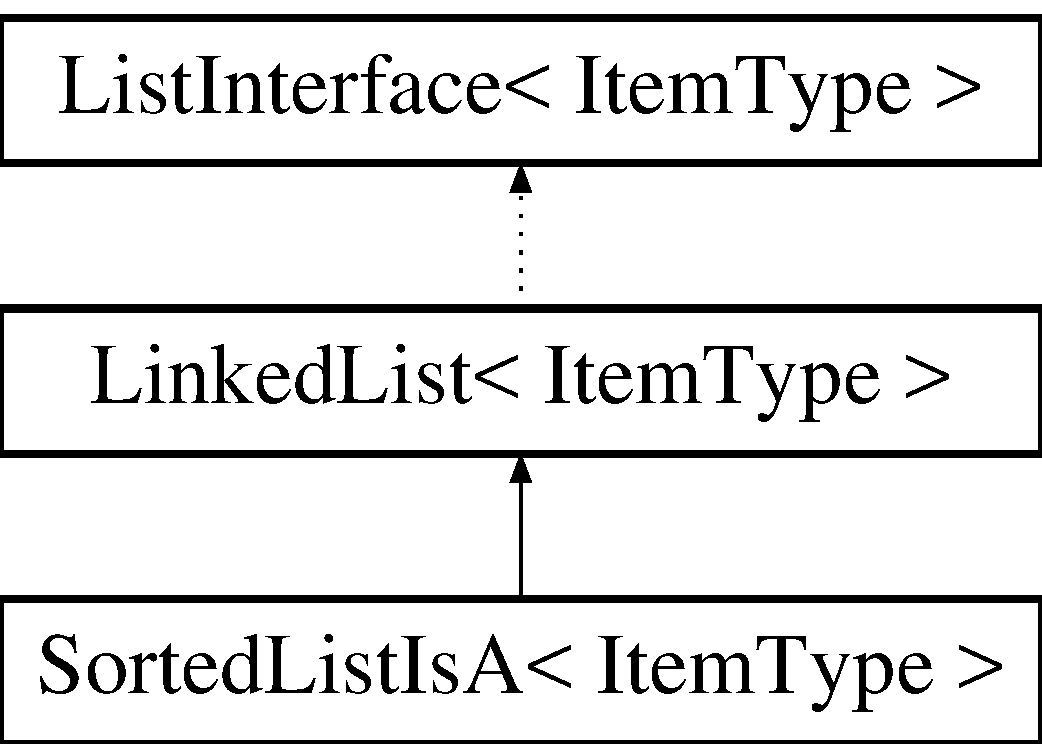
\includegraphics[height=3.000000cm]{class_sorted_list_is_a}
\end{center}
\end{figure}
\subsubsection*{Public Member Functions}
\begin{DoxyCompactItemize}
\item 
{\bfseries Sorted\+List\+IsA} (const \hyperlink{class_sorted_list_is_a}{Sorted\+List\+IsA}$<$ Item\+Type $>$ \&s\+List)\hypertarget{class_sorted_list_is_a_aaec289770ce0896fc13634fc370a095e}{}\label{class_sorted_list_is_a_aaec289770ce0896fc13634fc370a095e}

\item 
bool {\bfseries insert\+Sorted} (const Item\+Type \&new\+Entry)\hypertarget{class_sorted_list_is_a_a2b9ddfb2a19090085495518681de9b3f}{}\label{class_sorted_list_is_a_a2b9ddfb2a19090085495518681de9b3f}

\item 
bool {\bfseries remove\+Sorted} (int position)\hypertarget{class_sorted_list_is_a_ad8b46e67b19a7188c75491b1ad4bc152}{}\label{class_sorted_list_is_a_ad8b46e67b19a7188c75491b1ad4bc152}

\item 
int {\bfseries get\+Position} (const Item\+Type \&an\+Entry) const \hypertarget{class_sorted_list_is_a_a0fb1533091f08f88a73cd40f460a20c7}{}\label{class_sorted_list_is_a_a0fb1533091f08f88a73cd40f460a20c7}

\item 
bool \hyperlink{class_sorted_list_is_a_aa80ef5215183e3a17f2a2f2e76d4fca3}{insert} (int new\+Position, const Item\+Type \&new\+Entry) override
\item 
void \hyperlink{class_sorted_list_is_a_ae85cca0f8a4a306d6d28cc5993e5895c}{replace} (int position, const Item\+Type \&new\+Entry) override  throw (\+Precond\+Violated\+Except)
\end{DoxyCompactItemize}


\subsubsection{Member Function Documentation}
\index{Sorted\+List\+IsA@{Sorted\+List\+IsA}!insert@{insert}}
\index{insert@{insert}!Sorted\+List\+IsA@{Sorted\+List\+IsA}}
\paragraph[{\texorpdfstring{insert(int new\+Position, const Item\+Type \&new\+Entry) override}{insert(int newPosition, const ItemType &newEntry) override}}]{\setlength{\rightskip}{0pt plus 5cm}template$<$class Item\+Type $>$ bool {\bf Sorted\+List\+IsA}$<$ Item\+Type $>$\+::insert (
\begin{DoxyParamCaption}
\item[{int}]{new\+Position, }
\item[{const Item\+Type \&}]{new\+Entry}
\end{DoxyParamCaption}
)\hspace{0.3cm}{\ttfamily [override]}, {\ttfamily [virtual]}}\hypertarget{class_sorted_list_is_a_aa80ef5215183e3a17f2a2f2e76d4fca3}{}\label{class_sorted_list_is_a_aa80ef5215183e3a17f2a2f2e76d4fca3}
inserts an entry into the list at a given position \begin{DoxyPrecond}{Precondition}
None. 
\end{DoxyPrecond}
\begin{DoxyPostcond}{Postcondition}
if the position is valid and insertion is possible a new entry is entered into the list. 
\end{DoxyPostcond}

\begin{DoxyParams}{Parameters}
{\em new\+Position} & the position in the list at which to insert the new entry. \\
\hline
{\em new\+Entry} & the new item to be placed in the list. \\
\hline
\end{DoxyParams}
\begin{DoxyReturn}{Returns}
True if the item was successfully placed in the list. 
\end{DoxyReturn}


Reimplemented from \hyperlink{class_linked_list_ae8a19375505e87e2e4fc0e9b5afe4d4d}{Linked\+List$<$ Item\+Type $>$}.

\index{Sorted\+List\+IsA@{Sorted\+List\+IsA}!replace@{replace}}
\index{replace@{replace}!Sorted\+List\+IsA@{Sorted\+List\+IsA}}
\paragraph[{\texorpdfstring{replace(int position, const Item\+Type \&new\+Entry) override}{replace(int position, const ItemType &newEntry) override}}]{\setlength{\rightskip}{0pt plus 5cm}template$<$class Item\+Type $>$ void {\bf Sorted\+List\+IsA}$<$ Item\+Type $>$\+::replace (
\begin{DoxyParamCaption}
\item[{int}]{position, }
\item[{const Item\+Type \&}]{new\+Entry}
\end{DoxyParamCaption}
) throw  {\bf Precond\+Violated\+Except}) \hspace{0.3cm}{\ttfamily [override]}, {\ttfamily [virtual]}}\hypertarget{class_sorted_list_is_a_ae85cca0f8a4a306d6d28cc5993e5895c}{}\label{class_sorted_list_is_a_ae85cca0f8a4a306d6d28cc5993e5895c}
Replaces the entry at the given position in this list. \begin{DoxyPrecond}{Precondition}
1 $<$= position $<$= \hyperlink{class_linked_list_adae55d6b79235c816cb9e05027fd2e7a}{get\+Length()}. 
\end{DoxyPrecond}
\begin{DoxyPostcond}{Postcondition}
The entry at the given position is new\+Entry. 
\end{DoxyPostcond}

\begin{DoxyParams}{Parameters}
{\em position} & The list position of the entry to replace. \\
\hline
{\em new\+Entry} & The replacement entry. \\
\hline
\end{DoxyParams}

\begin{DoxyExceptions}{Exceptions}
{\em \hyperlink{class_precond_violated_except}{Precond\+Violated\+Except}} & if position $<$ 1 or position $>$ \hyperlink{class_linked_list_adae55d6b79235c816cb9e05027fd2e7a}{get\+Length()}. \\
\hline
\end{DoxyExceptions}


Reimplemented from \hyperlink{class_linked_list_a3035f880c50e7d8f68e67c093d4607ca}{Linked\+List$<$ Item\+Type $>$}.



The documentation for this class was generated from the following files\+:\begin{DoxyCompactItemize}
\item 
\hyperlink{_sorted_list_is_a_8h}{Sorted\+List\+Is\+A.\+h}\item 
Sorted\+List\+Is\+A.\+cpp\end{DoxyCompactItemize}

\section{File Documentation}
\hypertarget{_array_queue_8cpp}{}\subsection{Array\+Queue.\+cpp File Reference}
\label{_array_queue_8cpp}\index{Array\+Queue.\+cpp@{Array\+Queue.\+cpp}}
{\ttfamily \#include \char`\"{}Array\+Queue.\+h\char`\"{}}\\*


\subsubsection{Detailed Description}
A\+DT queue\+: Circular array-\/based implementation. 
\hypertarget{_array_queue_8h}{}\subsection{Array\+Queue.\+h File Reference}
\label{_array_queue_8h}\index{Array\+Queue.\+h@{Array\+Queue.\+h}}
{\ttfamily \#include \char`\"{}Queue\+Interface.\+h\char`\"{}}\\*
{\ttfamily \#include \char`\"{}Precond\+Violated\+Except.\+h\char`\"{}}\\*
{\ttfamily \#include \char`\"{}Array\+Queue.\+cpp\char`\"{}}\\*
\subsubsection*{Classes}
\begin{DoxyCompactItemize}
\item 
class \hyperlink{class_array_queue}{Array\+Queue$<$ Item\+Type $>$}
\end{DoxyCompactItemize}


\subsubsection{Detailed Description}
A\+DT queue\+: Circular array-\/based implementation. 
\hypertarget{_linked_list_8cpp}{}\subsection{Linked\+List.\+cpp File Reference}
\label{_linked_list_8cpp}\index{Linked\+List.\+cpp@{Linked\+List.\+cpp}}
{\ttfamily \#include \char`\"{}Linked\+List.\+h\char`\"{}}\\*
{\ttfamily \#include \char`\"{}Node.\+h\char`\"{}}\\*
{\ttfamily \#include \char`\"{}Precond\+Violated\+Except.\+h\char`\"{}}\\*


\subsubsection{Detailed Description}
A\+DT list\+: Link-\/based implementation. 
\hypertarget{_linked_list_8h}{\subsection{Linked\-List.\-h File Reference}
\label{_linked_list_8h}\index{Linked\-List.\-h@{Linked\-List.\-h}}
}


Header file for a linked list.  


{\ttfamily \#include \char`\"{}List\-Interface.\-h\char`\"{}}\\*
{\ttfamily \#include \char`\"{}Node.\-h\char`\"{}}\\*
{\ttfamily \#include \char`\"{}Precond\-Violated\-Except.\-h\char`\"{}}\\*
{\ttfamily \#include \char`\"{}Linked\-List.\-cpp\char`\"{}}\\*
\subsubsection*{Classes}
\begin{DoxyCompactItemize}
\item 
class \hyperlink{class_linked_list}{Linked\-List$<$ Item\-Type $>$}
\end{DoxyCompactItemize}


\subsubsection{Detailed Description}
Header file for a linked list. A\-D\-T list\-: Link-\/based implementation. Listing 9-\/2.

establishes functions for list  Created by Frank M. Carrano and Timothy M. Henry. Copyright (c) 2017 Pearson Education, Hoboken, New Jersey. 
\hypertarget{_linked_queue_8h}{}\subsection{Linked\+Queue.\+h File Reference}
\label{_linked_queue_8h}\index{Linked\+Queue.\+h@{Linked\+Queue.\+h}}
{\ttfamily \#include \char`\"{}Queue\+Interface.\+h\char`\"{}}\\*
{\ttfamily \#include \char`\"{}Node.\+h\char`\"{}}\\*
{\ttfamily \#include \char`\"{}Precond\+Violated\+Except.\+h\char`\"{}}\\*
{\ttfamily \#include $<$memory$>$}\\*
{\ttfamily \#include \char`\"{}Linked\+Queue.\+cpp\char`\"{}}\\*
\subsubsection*{Classes}
\begin{DoxyCompactItemize}
\item 
class \hyperlink{class_linked_queue}{Linked\+Queue$<$ Item\+Type $>$}
\end{DoxyCompactItemize}


\subsubsection{Detailed Description}
A\+DT queue\+: Link-\/based implementation. 
\hypertarget{_list_interface_8h}{\subsection{List\-Interface.\-h File Reference}
\label{_list_interface_8h}\index{List\-Interface.\-h@{List\-Interface.\-h}}
}


Interface file for the List A\-D\-T.  


\subsubsection*{Classes}
\begin{DoxyCompactItemize}
\item 
class \hyperlink{class_list_interface}{List\-Interface$<$ Item\-Type $>$}
\end{DoxyCompactItemize}


\subsubsection{Detailed Description}
Interface file for the List A\-D\-T. \begin{DoxyAuthor}{Author}
Rory Pierce
\end{DoxyAuthor}
Specifies the implementation contract of the List A\-D\-T

\begin{DoxyVersion}{Version}
0.\-10
\end{DoxyVersion}
Adapted from Frank M. Carrano and Timothy M. Henry Copyright (c) 2017 Pearson Education, Hoboken, New Jersey. 
\hypertarget{_node_8cpp}{\subsection{Node.\-cpp File Reference}
\label{_node_8cpp}\index{Node.\-cpp@{Node.\-cpp}}
}
{\ttfamily \#include \char`\"{}Node.\-h\char`\"{}}\\*


\subsubsection{Detailed Description}
Listing 4-\/2 
\hypertarget{_node_8h}{\subsection{Node.\-h File Reference}
\label{_node_8h}\index{Node.\-h@{Node.\-h}}
}
{\ttfamily \#include \char`\"{}Node.\-cpp\char`\"{}}\\*
\subsubsection*{Classes}
\begin{DoxyCompactItemize}
\item 
class \hyperlink{class_node}{Node$<$ Item\-Type $>$}
\end{DoxyCompactItemize}


\subsubsection{Detailed Description}
Listing 4-\/1 
\hypertarget{_precond_violated_except_8cpp}{\subsection{Precond\-Violated\-Except.\-cpp File Reference}
\label{_precond_violated_except_8cpp}\index{Precond\-Violated\-Except.\-cpp@{Precond\-Violated\-Except.\-cpp}}
}
{\ttfamily \#include \char`\"{}Precond\-Violated\-Except.\-h\char`\"{}}\\*


\subsubsection{Detailed Description}
Listing 7-\/6. 
\hypertarget{_precond_violated_except_8h}{}\subsection{Precond\+Violated\+Except.\+h File Reference}
\label{_precond_violated_except_8h}\index{Precond\+Violated\+Except.\+h@{Precond\+Violated\+Except.\+h}}
{\ttfamily \#include $<$stdexcept$>$}\\*
{\ttfamily \#include $<$string$>$}\\*
\subsubsection*{Classes}
\begin{DoxyCompactItemize}
\item 
class \hyperlink{class_precond_violated_except}{Precond\+Violated\+Except}
\end{DoxyCompactItemize}


\subsubsection{Detailed Description}
Listing 7-\/5. 
\hypertarget{_priority_queue_interface_8h}{}\subsection{Priority\+Queue\+Interface.\+h File Reference}
\label{_priority_queue_interface_8h}\index{Priority\+Queue\+Interface.\+h@{Priority\+Queue\+Interface.\+h}}
\subsubsection*{Classes}
\begin{DoxyCompactItemize}
\item 
class \hyperlink{class_priority_queue_interface}{Priority\+Queue\+Interface$<$ Item\+Type $>$}
\end{DoxyCompactItemize}

\hypertarget{_queue_interface_8h}{}\subsection{Queue\+Interface.\+h File Reference}
\label{_queue_interface_8h}\index{Queue\+Interface.\+h@{Queue\+Interface.\+h}}
\subsubsection*{Classes}
\begin{DoxyCompactItemize}
\item 
class \hyperlink{class_queue_interface}{Queue\+Interface$<$ Item\+Type $>$}
\end{DoxyCompactItemize}

\hypertarget{_s_l___priority_queue_8h}{}\subsection{S\+L\+\_\+\+Priority\+Queue.\+h File Reference}
\label{_s_l___priority_queue_8h}\index{S\+L\+\_\+\+Priority\+Queue.\+h@{S\+L\+\_\+\+Priority\+Queue.\+h}}
{\ttfamily \#include \char`\"{}Priority\+Queue\+Interface.\+h\char`\"{}}\\*
{\ttfamily \#include \char`\"{}Sorted\+List\+Is\+A.\+h\char`\"{}}\\*
{\ttfamily \#include \char`\"{}Precond\+Violated\+Except.\+h\char`\"{}}\\*
{\ttfamily \#include $<$memory$>$}\\*
{\ttfamily \#include \char`\"{}S\+L\+\_\+\+Priority\+Queue.\+cpp\char`\"{}}\\*
\subsubsection*{Classes}
\begin{DoxyCompactItemize}
\item 
class \hyperlink{class_s_l___priority_queue}{S\+L\+\_\+\+Priority\+Queue$<$ Item\+Type $>$}
\end{DoxyCompactItemize}


\subsubsection{Detailed Description}
A\+DT priority queue\+: A\+DT sorted list implementation. 
\hypertarget{_sorted_list_interface_8h}{}\subsection{Sorted\+List\+Interface.\+h File Reference}
\label{_sorted_list_interface_8h}\index{Sorted\+List\+Interface.\+h@{Sorted\+List\+Interface.\+h}}
\subsubsection*{Classes}
\begin{DoxyCompactItemize}
\item 
class \hyperlink{class_sorted_list_interface}{Sorted\+List\+Interface$<$ Item\+Type $>$}
\end{DoxyCompactItemize}


\subsubsection{Detailed Description}
Interface for the A\+DT sorted list 
\hypertarget{_sorted_list_is_a_8h}{}\subsection{Sorted\+List\+Is\+A.\+h File Reference}
\label{_sorted_list_is_a_8h}\index{Sorted\+List\+Is\+A.\+h@{Sorted\+List\+Is\+A.\+h}}
{\ttfamily \#include $<$memory$>$}\\*
{\ttfamily \#include \char`\"{}Linked\+List.\+h\char`\"{}}\\*
{\ttfamily \#include \char`\"{}Node.\+h\char`\"{}}\\*
{\ttfamily \#include \char`\"{}Precond\+Violated\+Except.\+h\char`\"{}}\\*
{\ttfamily \#include \char`\"{}Sorted\+List\+Is\+A.\+cpp\char`\"{}}\\*
\subsubsection*{Classes}
\begin{DoxyCompactItemize}
\item 
class \hyperlink{class_sorted_list_is_a}{Sorted\+List\+Is\+A$<$ Item\+Type $>$}
\end{DoxyCompactItemize}


\subsubsection{Detailed Description}
A\+DT sorted list using A\+DT list. 
%--- End generated contents ---

% Index
\newpage
\phantomsection
\clearemptydoublepage
\addcontentsline{toc}{section}{Index}
\printindex

\end{document}
